\documentclass[
  man,
  floatsintext,
  longtable,
  nolmodern,
  notxfonts,
  notimes,
  colorlinks=true,linkcolor=blue,citecolor=blue,urlcolor=blue]{apa7}

\usepackage{amsmath}
\usepackage{amssymb}


\geometry{landscape,margin=1in}
\fancyhfoffset[LE,RO]{0cm}


\RequirePackage{longtable}
\RequirePackage{threeparttablex}

\makeatletter
\renewcommand{\paragraph}{\@startsection{paragraph}{4}{\parindent}%
	{0\baselineskip \@plus 0.2ex \@minus 0.2ex}%
	{-.5em}%
	{\normalfont\normalsize\bfseries\typesectitle}}

\renewcommand{\subparagraph}[1]{\@startsection{subparagraph}{5}{0.5em}%
	{0\baselineskip \@plus 0.2ex \@minus 0.2ex}%
	{-\z@\relax}%
	{\normalfont\normalsize\bfseries\itshape\hspace{\parindent}{#1}\textit{\addperi}}{\relax}}
\makeatother




\usepackage{longtable, booktabs, multirow, multicol, colortbl, hhline, caption, array, float, xpatch}
\usepackage{subcaption}


\renewcommand\thesubfigure{\Alph{subfigure}}
\setcounter{topnumber}{2}
\setcounter{bottomnumber}{2}
\setcounter{totalnumber}{4}
\renewcommand{\topfraction}{0.85}
\renewcommand{\bottomfraction}{0.85}
\renewcommand{\textfraction}{0.15}
\renewcommand{\floatpagefraction}{0.7}

\usepackage{tcolorbox}
\tcbuselibrary{listings,theorems, breakable, skins}
\usepackage{fontawesome5}

\definecolor{quarto-callout-color}{HTML}{909090}
\definecolor{quarto-callout-note-color}{HTML}{0758E5}
\definecolor{quarto-callout-important-color}{HTML}{CC1914}
\definecolor{quarto-callout-warning-color}{HTML}{EB9113}
\definecolor{quarto-callout-tip-color}{HTML}{00A047}
\definecolor{quarto-callout-caution-color}{HTML}{FC5300}
\definecolor{quarto-callout-color-frame}{HTML}{ACACAC}
\definecolor{quarto-callout-note-color-frame}{HTML}{4582EC}
\definecolor{quarto-callout-important-color-frame}{HTML}{D9534F}
\definecolor{quarto-callout-warning-color-frame}{HTML}{F0AD4E}
\definecolor{quarto-callout-tip-color-frame}{HTML}{02B875}
\definecolor{quarto-callout-caution-color-frame}{HTML}{FD7E14}

%\newlength\Oldarrayrulewidth
%\newlength\Oldtabcolsep


\usepackage{hyperref}




\providecommand{\tightlist}{%
  \setlength{\itemsep}{0pt}\setlength{\parskip}{0pt}}
\usepackage{longtable,booktabs,array}
\newcounter{none} % for unnumbered tables
\usepackage{calc} % for calculating minipage widths
% Correct order of tables after \paragraph or \subparagraph
\usepackage{etoolbox}
\makeatletter
\patchcmd\longtable{\par}{\if@noskipsec\mbox{}\fi\par}{}{}
\makeatother
% Allow footnotes in longtable head/foot
\IfFileExists{footnotehyper.sty}{\usepackage{footnotehyper}}{\usepackage{footnote}}
\makesavenoteenv{longtable}

\usepackage{graphicx}
\makeatletter
\newsavebox\pandoc@box
\newcommand*\pandocbounded[1]{% scales image to fit in text height/width
  \sbox\pandoc@box{#1}%
  \Gscale@div\@tempa{\textheight}{\dimexpr\ht\pandoc@box+\dp\pandoc@box\relax}%
  \Gscale@div\@tempb{\linewidth}{\wd\pandoc@box}%
  \ifdim\@tempb\p@<\@tempa\p@\let\@tempa\@tempb\fi% select the smaller of both
  \ifdim\@tempa\p@<\p@\scalebox{\@tempa}{\usebox\pandoc@box}%
  \else\usebox{\pandoc@box}%
  \fi%
}
% Set default figure placement to htbp
\def\fps@figure{htbp}
\makeatother


% definitions for citeproc citations
\NewDocumentCommand\citeproctext{}{}
\NewDocumentCommand\citeproc{mm}{%
  \begingroup\def\citeproctext{#2}\cite{#1}\endgroup}
\makeatletter
 % allow citations to break across lines
 \let\@cite@ofmt\@firstofone
 % avoid brackets around text for \cite:
 \def\@biblabel#1{}
 \def\@cite#1#2{{#1\if@tempswa , #2\fi}}
\makeatother
\newlength{\cslhangindent}
\setlength{\cslhangindent}{1.5em}
\newlength{\csllabelwidth}
\setlength{\csllabelwidth}{3em}
\newenvironment{CSLReferences}[2] % #1 hanging-indent, #2 entry-spacing
 {\begin{list}{}{%
  \setlength{\itemindent}{0pt}
  \setlength{\leftmargin}{0pt}
  \setlength{\parsep}{0pt}
  % turn on hanging indent if param 1 is 1
  \ifodd #1
   \setlength{\leftmargin}{\cslhangindent}
   \setlength{\itemindent}{-1\cslhangindent}
  \fi
  % set entry spacing
  \setlength{\itemsep}{#2\baselineskip}}}
 {\end{list}}
\usepackage{calc}
\newcommand{\CSLBlock}[1]{\hfill\break\parbox[t]{\linewidth}{\strut\ignorespaces#1\strut}}
\newcommand{\CSLLeftMargin}[1]{\parbox[t]{\csllabelwidth}{\strut#1\strut}}
\newcommand{\CSLRightInline}[1]{\parbox[t]{\linewidth - \csllabelwidth}{\strut#1\strut}}
\newcommand{\CSLIndent}[1]{\hspace{\cslhangindent}#1}





\usepackage{newtx}

\defaultfontfeatures{Scale=MatchLowercase}
\defaultfontfeatures[\rmfamily]{Ligatures=TeX,Scale=1}





\title{Supplement A - Technical Details for The Link Function Problem in
Psychological Interaction Testing}


\shorttitle{Supplement A - Technical Details for The Link Function
Problem in Psychological Interaction Testing}


\usepackage{etoolbox}









\authorsnames[{1},{2},{1},{1},{1}]{Margherita Calderan,Filippo
Gambarota,Laura Sità,Tommaso Feraco,Enrico Toffalini}







\authorsaffiliations{
{Department of General Psychology, University of Padova},{Department of
Developmental Psychology and Socialization, University of Padova}}




\leftheader{Calderan, Gambarota, Sità, Feraco and Toffalini}






\authornote{\par{\addORCIDlink{Margherita
Calderan}{0009-0005-5668-5162}}\par{\addORCIDlink{Filippo
Gambarota}{0000-0002-6666-1747}}\par{\addORCIDlink{Laura
Sità}{0009-0000-6017-9979}}\par{\addORCIDlink{Tommaso
Feraco}{0000-0002-8920-5330}}\par{\addORCIDlink{Enrico
Toffalini}{0000-0002-1404-5133}} 
\par{ }
\par{       }
\par{Correspondence concerning this article should be addressed
to Enrico Toffalini, Department of General Psychology, University of
Padova, Via Venezia
8, Padova 35131, Italy, Email: \href{mailto:enrico.toffalini@unipd.it}{enrico.toffalini@unipd.it}}
}

\makeatletter
\let\endoldlt\endlongtable
\def\endlongtable{
\hline
\endoldlt
}
\makeatother

\urlstyle{same}



% Table typography: wrapped lines inside a cell are set slightly tighter
% than normal and each row gets a little extra vertical air, so a line
% break inside a cell is not mistaken for the start of a new table row.
\usepackage{etoolbox}
\usepackage{array}
\AtBeginEnvironment{longtable}{%
  \linespread{0.95}\selectfont
  \setlength{\extrarowheight}{6pt}}
\AtBeginEnvironment{tabular}{%
  \linespread{0.95}\selectfont
  \setlength{\extrarowheight}{6pt}}
\usepackage{float}
\makeatletter
\@ifpackageloaded{caption}{}{\usepackage{caption}}
\AtBeginDocument{%
\ifdefined\contentsname
  \renewcommand*\contentsname{Table of contents}
\else
  \newcommand\contentsname{Table of contents}
\fi
\ifdefined\listfigurename
  \renewcommand*\listfigurename{List of Figures}
\else
  \newcommand\listfigurename{List of Figures}
\fi
\ifdefined\listtablename
  \renewcommand*\listtablename{List of Tables}
\else
  \newcommand\listtablename{List of Tables}
\fi
\ifdefined\figurename
  \renewcommand*\figurename{Figure}
\else
  \newcommand\figurename{Figure}
\fi
\ifdefined\tablename
  \renewcommand*\tablename{Table}
\else
  \newcommand\tablename{Table}
\fi
}
\@ifpackageloaded{float}{}{\usepackage{float}}
\floatstyle{ruled}
\@ifundefined{c@chapter}{\newfloat{codelisting}{h}{lop}}{\newfloat{codelisting}{h}{lop}[chapter]}
\floatname{codelisting}{Listing}
\newcommand*\listoflistings{\listof{codelisting}{List of Listings}}
\makeatother
\makeatletter
\makeatother
\makeatletter
\@ifpackageloaded{caption}{}{\usepackage{caption}}
\@ifpackageloaded{subcaption}{}{\usepackage{subcaption}}
\makeatother

% From https://tex.stackexchange.com/a/645996/211326
%%% apa7 doesn't want to add appendix section titles in the toc
%%% let's make it do it
\makeatletter
\xpatchcmd{\appendix}
  {\par}
  {\addcontentsline{toc}{section}{\@currentlabelname}\par}
  {}{}
\makeatother

%% Disable longtable counter
%% https://tex.stackexchange.com/a/248395/211326

\usepackage{etoolbox}

\makeatletter
\patchcmd{\LT@caption}
  {\bgroup}
  {\bgroup\global\LTpatch@captiontrue}
  {}{}
\patchcmd{\longtable}
  {\par}
  {\par\global\LTpatch@captionfalse}
  {}{}
\apptocmd{\endlongtable}
  {\ifLTpatch@caption\else\addtocounter{table}{-1}\fi}
  {}{}
\newif\ifLTpatch@caption
\makeatother

\begin{document}

\maketitle


\hypertarget{toc}{}
\tableofcontents
\newpage
\section[Introduction]{Supplement A - Technical Details for The Link
Function Problem in Psychological Interaction Testing}


\setlength\LTleft{0pt}




\section{S1. Scope of this
supplement}\label{s1.-scope-of-this-supplement}

This supplement reports extended review methods and reliability,
followed by the chance-corrected-link algebra and the generative
parameters behind the illustrative figures. It then gives full
specifications and estimation details for the three worked simulations
and the diagnostic simulation, together with supplementary results.

\section{S2. Preregistered review: extended methods and
reliability}\label{s2.-preregistered-review-extended-methods-and-reliability}

\subsection{Protocol and sampling
frame}\label{protocol-and-sampling-frame}

The review protocol was preregistered before any record was screened and
is available at \url{https://osf.io/bdu73/}, together with the coding
data dictionary. The protocol specified a descriptive review of recent
psychological research articles from five pre-specified journals, one
per major area: \emph{Psychological Science} (general), \emph{Journal of
Experimental Psychology: General} (experimental), \emph{Journal of
Personality and Social Psychology} (social), \emph{Developmental
Science} (developmental), and \emph{Psychological Medicine} (clinical).
Journals were selected on a discretionary combination of criteria stated
in the protocol: first-quartile Impact Factor in the 2023 Journal
Citation Reports, not primarily publishing reviews, not narrowly
specialized, and strong general reputation in the respective field, as
jointly evaluated by the coauthors.

Article records were retrieved from Elsevier's Scopus database for all
articles published in these journals in 2024. For each journal, the full
record list was randomly ordered and then screened in that order until
40 eligible articles testing at least one interaction on an observed
outcome were included, yielding 200 coded articles across the five
journals. The preregistered stopping rule referred to
interaction-testing articles in general; the restriction to observed
outcomes was introduced during implementation and is a protocol
deviation described below. Screening a larger set also allowed
estimating the proportion of eligible empirical articles that test
interactions. The design is targeted and descriptive: it characterizes
reporting practice in influential outlets during the sampled year. It is
not a random or stratified sample of all psychology journals, and the
estimates are not prevalence estimates for the discipline.

\subsection{Eligibility and coding
workflow}\label{eligibility-and-coding-workflow}

Eligible articles were empirical articles presenting original
psychological research. The following were excluded, per protocol:
reviews and meta-analyses; editorials, commentaries, opinion papers, and
theoretical articles without empirical data; qualitative-only articles;
replication-only studies; and psychometric validation studies. Articles
were coded in detail only if they tested at least one interaction,
through statistical modeling or ANOVA. Analyzing latent variables or
fitting structural equation models was not in itself a reason for
exclusion. Because our family and link coding was defined for observed
outcomes, articles whose interaction tests all concerned latent outcomes
(for example, latent moderation in a structural equation model, or
moderation of latent variance components in a twin model) were recorded
as eligible and interaction-testing, but were not coded in detail and
did not count toward the 40 articles per journal. The preregistration
did not specify this restriction, so we treat it as a protocol
deviation. It was applied during screening, and we retained the
resulting sample rather than reconstructing the point at which screening
would otherwise have stopped. Articles combining latent-variable
analyses with at least one observed-outcome interaction were coded, with
the coding restricted to their observed-outcome interactions.

The resulting screening flow is reported in
Table~\ref{tbl-screening-flow}.

\begin{longtable}[]{@{}
  >{\raggedright\arraybackslash}p{(\linewidth - 2\tabcolsep) * \real{0.9438}}
  >{\raggedleft\arraybackslash}p{(\linewidth - 2\tabcolsep) * \real{0.0562}}@{}}
\caption{Screening flow for the preregistered
review.}\label{tbl-screening-flow}\tabularnewline
\toprule\noalign{}
\begin{minipage}[b]{\linewidth}\raggedright
Step
\end{minipage} & \begin{minipage}[b]{\linewidth}\raggedleft
N
\end{minipage} \\
\midrule\noalign{}
\endfirsthead
\toprule\noalign{}
\begin{minipage}[b]{\linewidth}\raggedright
Step
\end{minipage} & \begin{minipage}[b]{\linewidth}\raggedleft
N
\end{minipage} \\
\midrule\noalign{}
\endhead
\bottomrule\noalign{}
\endlastfoot
records retrieved across journal sheets & 2175 \\
articles screened for eligibility & 367 \\
eligible empirical articles & 345 \\
eligible articles testing at least one interaction & 208 \\
eligible articles not testing interactions & 137 \\
interaction-testing articles with at least one observed-outcome
interaction (coded) & 200 \\
interaction-testing articles with interactions on latent outcomes only &
8 \\
\end{longtable}

Each of the 200 coded articles was independently coded by two
researchers. Discrepancies were resolved through discussion or, if
needed, by consulting the other coauthors. Generative AI tools were used
only as an optional aid to locate relevant passages within an article;
all coding used in the review is human.

\begin{longtable}[]{@{}
  >{\raggedright\arraybackslash}p{(\linewidth - 4\tabcolsep) * \real{0.1579}}
  >{\raggedright\arraybackslash}p{(\linewidth - 4\tabcolsep) * \real{0.6842}}
  >{\raggedright\arraybackslash}p{(\linewidth - 4\tabcolsep) * \real{0.1579}}@{}}
\caption{Coded variables and their preregistered
definitions.}\label{tbl-variables}\tabularnewline
\toprule\noalign{}
\begin{minipage}[b]{\linewidth}\raggedright
Variable
\end{minipage} & \begin{minipage}[b]{\linewidth}\raggedright
Definition (preregistered)
\end{minipage} & \begin{minipage}[b]{\linewidth}\raggedright
Type
\end{minipage} \\
\midrule\noalign{}
\endfirsthead
\toprule\noalign{}
\begin{minipage}[b]{\linewidth}\raggedright
Variable
\end{minipage} & \begin{minipage}[b]{\linewidth}\raggedright
Definition (preregistered)
\end{minipage} & \begin{minipage}[b]{\linewidth}\raggedright
Type
\end{minipage} \\
\midrule\noalign{}
\endhead
\bottomrule\noalign{}
\endlastfoot
Tests interactions & Whether the article tests at least one interaction
term in a statistical model or using an ANOVA. & Boolean \\
Uses non identity link function & Whether at least one tested
interaction is presumably analyzed with a non-identity link function
(for example, because a generalized linear model was used). & Boolean \\
Explicit link function & Whether the link function is explicitly
declared for at least one statistical model in the article. Indicating
only which generalized linear model or family was used is not enough. &
Boolean \\
Incorrect identity link function & Whether at least one tested
interaction is analyzed using an identity link function when another,
non-identity link function would be more appropriate. & Boolean \\
Finds significant interactions & Whether at least one interaction, among
those where the link was coded as incorrectly identity, yields a
statistically significant result, or is considered and discussed
analogously in non-frequentist analyses. & Boolean \\
Response variable types & Non-exclusive list of response-variable types
on which interactions are tested (for example, sum score, accuracy,
error count, response times, ordinal/Likert). & Category \\
\end{longtable}

Beyond these definitions, the coders applied a small set of operational
rules for the recurring borderline decisions.
Table~\ref{tbl-coding-rules} records the ones that most affect the
reported counts.

\begin{longtable}[]{@{}
  >{\raggedright\arraybackslash}p{(\linewidth - 4\tabcolsep) * \real{0.1111}}
  >{\raggedright\arraybackslash}p{(\linewidth - 4\tabcolsep) * \real{0.4444}}
  >{\raggedright\arraybackslash}p{(\linewidth - 4\tabcolsep) * \real{0.4444}}@{}}
\caption{Operational rules the coders applied for the decisions that
most affect the reported counts, condensed from the coding sheet. The
preregistered variable definitions are in
Table~\ref{tbl-variables}.}\label{tbl-coding-rules}\tabularnewline
\toprule\noalign{}
\begin{minipage}[b]{\linewidth}\raggedright
Variable
\end{minipage} & \begin{minipage}[b]{\linewidth}\raggedright
Coded ``Yes'' when
\end{minipage} & \begin{minipage}[b]{\linewidth}\raggedright
Decisions that most affect the count
\end{minipage} \\
\midrule\noalign{}
\endfirsthead
\toprule\noalign{}
\begin{minipage}[b]{\linewidth}\raggedright
Variable
\end{minipage} & \begin{minipage}[b]{\linewidth}\raggedright
Coded ``Yes'' when
\end{minipage} & \begin{minipage}[b]{\linewidth}\raggedright
Decisions that most affect the count
\end{minipage} \\
\midrule\noalign{}
\endhead
\bottomrule\noalign{}
\endlastfoot
Non-identity link used & at least one tested interaction is fitted with
a model implying a non-identity link, that is, any GLM or GLMM beyond
the Gaussian-identity default (ANOVA, ordinary regression, linear mixed
model). & A model named ``logistic'', ``probit'', ``Poisson'',
``negative binomial'', ``ordinal''/``cumulative'', or ``Gamma''
regression implies a non-identity link. \\
Explicit link function & the link is identifiable from the report,
either stated in words or named through a link-specific model. &
``Logistic regression'' (logit), ``probit regression'' (probit), and
``Poisson'' or ``log-linear'' (log) count as explicit. Naming only a
family, a ``generalized linear model'', or a ``GLMM'' does not. \\
Gaussian-identity analysis on a constrained outcome & an interaction is
tested with an identity-link model (ANOVA, ordinary regression, linear
mixed model, or a test on cell means) applied to an outcome with formal
constraints: bounded, discrete, positive-only, or with a known chance
level. & Flagged only when the constraint is clear from the report. Not
flagged when the analysis is explicitly justified as an observed-score
estimand, or when the outcome is plausibly continuous and far from any
bound. \\
Significant interaction & at least one interaction already flagged as a
Gaussian-identity analysis on a constrained outcome is reported as
statistically significant, or is interpreted analogously (for example, a
credible interval excluding zero) in a Bayesian analysis. & Restricted
to interactions already flagged in the row above. \\
Response-variable types & --- & Non-exclusive: one article can
contribute several types (sum score, accuracy or proportion, error
count, response time, ordinal/Likert, neural or physiological,
difference score, correlation). \\
\end{longtable}

One additional decision beyond those summarized in
Table~\ref{tbl-coding-rules} concerned transformed outcomes. Coding
referred to the response on the scale on which it entered the model.
When authors transformed the outcome before applying a linear model or
ANOVA, the analysis was evaluated on the transformed scale and was not
flagged. For example, a linear model or ANOVA applied directly to raw
response times was flagged because response times are constrained to
positive values, whereas the same analysis applied to log transformed
response times was not. Logarithmic transformations were the most
common, but the same rule was applied to the other transformations
encountered in the reviewed articles.

Two notes clarify the interpretation of the coding variables. First,
\emph{Incorrect identity link function} is a conservative screening flag
for a formal mismatch between the observed-outcome constraints and the
identity-link generative model. Cases were flagged only when the
constraint was identifiable from the published report; when the report
did not allow this judgment, the case was not counted. The flag is not
an error rate, not a severity grade, and does not imply that the
substantive conclusion is false, since an observed-score estimand can be
a deliberate and defensible target. Second, \emph{Response variable
types} is non-exclusive: one article can contribute to several
categories, so the category counts do not sum to the number of articles.

The last coding variable is described in greater detail in
Table~\ref{tbl-response-variable-definitions}, which summarizes the
response variable labels used during coding and their relation to the
broader categories reported in the main paper. Classification was based
primarily on the process that generated the response rather than on the
terminology used by the article authors. When this process could not be
determined reliably from the report, the authors' terminology was
retained.

\begin{longtable}[]{@{}
  >{\raggedright\arraybackslash}p{(\linewidth - 4\tabcolsep) * \real{0.3333}}
  >{\raggedright\arraybackslash}p{(\linewidth - 4\tabcolsep) * \real{0.3333}}
  >{\raggedright\arraybackslash}p{(\linewidth - 4\tabcolsep) * \real{0.3333}}@{}}
\caption{Operational definitions of the broad response variable
categories reported in the main paper and their principal detailed
coding labels. An article could contribute to more than one
row.}\label{tbl-response-variable-definitions}\tabularnewline
\toprule\noalign{}
\begin{minipage}[b]{\linewidth}\raggedright
Broad category in the main paper
\end{minipage} & \begin{minipage}[b]{\linewidth}\raggedright
Principal detailed labels
\end{minipage} & \begin{minipage}[b]{\linewidth}\raggedright
Operational definition and coding decisions
\end{minipage} \\
\midrule\noalign{}
\endfirsthead
\toprule\noalign{}
\begin{minipage}[b]{\linewidth}\raggedright
Broad category in the main paper
\end{minipage} & \begin{minipage}[b]{\linewidth}\raggedright
Principal detailed labels
\end{minipage} & \begin{minipage}[b]{\linewidth}\raggedright
Operational definition and coding decisions
\end{minipage} \\
\midrule\noalign{}
\endhead
\bottomrule\noalign{}
\endlastfoot
Binary / accuracy / proportions & Binary; proportion & \emph{Binary}
indicated a finite number of discrete binary events, such as correct and
incorrect responses over a predetermined number of trials. This label
was retained when binary responses were summed or averaged.
\emph{Proportion} was reserved for responses treated as varying
continuously between 0 and 1 and not determined by a fixed number of
discrete binary events. Accuracy calculated over a predetermined number
of trials was therefore coded as binary rather than as a continuous
proportion. \\
Sum scores / composites & Sum score; log transformed sum score;
normalized sum score & A \emph{sum score} was a sum or average of
multiple ordinal or slider responses. Aggregates of dichotomous
responses were instead coded as binary. Log transformed and normalized
totals were identified separately during detailed coding but were
included in the same broad category for reporting. \\
Ordinal / Likert / ratings & Ordinal; slider & \emph{Ordinal} indicated
a single ordered response with no more than 10 response levels. A single
ordered response with more than 10 available levels was coded as a
\emph{slider}. When multiple ordinal or slider responses were summed or
averaged, the resulting outcome was coded as a sum score. \\
Response times / durations & Response time; log transformed response
time; inverse response time & Positive response or reaction times were
included in this category whether they were analyzed on their original
scale, after a logarithmic transformation, or after a reciprocal
transformation. The specific transformation was retained in the detailed
coding. \\
Neural / physiological measures & Amplitude; log transformed amplitude;
heart rate; heart rate variability; skin conductance response &
Continuous neural and physiological measurements were included in this
category. When a physiological response represented a count rather than
an amplitude or continuous measurement, it was classified according to
the process that generated the count. \\
Difference / distance scores & Difference score; distance & A
\emph{difference score} was the arithmetic difference between two
individual responses. \emph{Distance} referred to continuous distance
measures, including angular deviation, positional error, and geodesic
distance. \\
Counts / error counts & Count; log transformed count; frequency &
\emph{Count} was reserved for counts without a predetermined upper
bound. Counts of correct responses or errors over a fixed number of
trials were coded as binary because the number of possible events was
predetermined. Generic descriptions such as ``errors'' were therefore
classified according to the underlying process whenever it could be
established from the report. \\
Correlations / associations & Correlation; Fisher z transformed
correlation & Correlations used as outcomes and their Fisher z
transformations were distinguished during detailed coding and combined
in this broad category for reporting. \\
\end{longtable}

Coding relied only on what a reader can observe in a published report:
the analysis described, the outcome described, and any explicit
statement of family or link. The review therefore documents reporting
practice, not the correctness of substantive conclusions. For the same
reason, the review did not classify interactions as removable or
nonremovable at the article level, because published reports rarely
provide the target contrast, the complete coefficients, and the assumed
measurement scale that such a classification requires.

\subsection{Interrater agreement}\label{interrater-agreement}

Double-coded records with complete coder pairs are summarized in
Table~\ref{tbl-agreement}, with raw percentage agreement and Cohen's
kappa reported together. Several coded variables had imbalanced marginal
distributions, a setting in which kappa can be conservative, so the
coder-specific yes rates are reported alongside to let readers evaluate
the agreement pattern directly.

\begin{longtable}[]{@{}
  >{\raggedright\arraybackslash}p{(\linewidth - 10\tabcolsep) * \real{0.4211}}
  >{\raggedleft\arraybackslash}p{(\linewidth - 10\tabcolsep) * \real{0.0526}}
  >{\raggedright\arraybackslash}p{(\linewidth - 10\tabcolsep) * \real{0.1316}}
  >{\raggedright\arraybackslash}p{(\linewidth - 10\tabcolsep) * \real{0.0789}}
  >{\raggedright\arraybackslash}p{(\linewidth - 10\tabcolsep) * \real{0.1579}}
  >{\raggedright\arraybackslash}p{(\linewidth - 10\tabcolsep) * \real{0.1579}}@{}}
\caption{Interrater agreement for double-coded
records.}\label{tbl-agreement}\tabularnewline
\toprule\noalign{}
\begin{minipage}[b]{\linewidth}\raggedright
Item
\end{minipage} & \begin{minipage}[b]{\linewidth}\raggedleft
N
\end{minipage} & \begin{minipage}[b]{\linewidth}\raggedright
Agreement
\end{minipage} & \begin{minipage}[b]{\linewidth}\raggedright
Kappa
\end{minipage} & \begin{minipage}[b]{\linewidth}\raggedright
Coder 1 yes
\end{minipage} & \begin{minipage}[b]{\linewidth}\raggedright
Coder 2 yes
\end{minipage} \\
\midrule\noalign{}
\endfirsthead
\toprule\noalign{}
\begin{minipage}[b]{\linewidth}\raggedright
Item
\end{minipage} & \begin{minipage}[b]{\linewidth}\raggedleft
N
\end{minipage} & \begin{minipage}[b]{\linewidth}\raggedright
Agreement
\end{minipage} & \begin{minipage}[b]{\linewidth}\raggedright
Kappa
\end{minipage} & \begin{minipage}[b]{\linewidth}\raggedright
Coder 1 yes
\end{minipage} & \begin{minipage}[b]{\linewidth}\raggedright
Coder 2 yes
\end{minipage} \\
\midrule\noalign{}
\endhead
\bottomrule\noalign{}
\endlastfoot
Uses non-identity link & 199 & 92.0\% & 0.81 & 28.1\% & 30.2\% \\
Explicit link reported & 199 & 88.9\% & 0.66 & 20.6\% & 20.6\% \\
Gaussian-identity flagged & 197 & 88.3\% & 0.71 & 71.6\% & 72.1\% \\
Significant flagged interaction & 141 & 91.5\% & 0.68 & 86.5\% &
82.3\% \\
\end{longtable}

\subsection{By-journal descriptives}\label{by-journal-descriptives}

Table~\ref{tbl-by-journal} reports the review descriptives by journal.
Link percentages are computed within the coded articles (eligible
articles with at least one observed-outcome interaction, 40 per
journal), whereas the interaction-testing percentage counts interactions
on observed or latent outcomes and is computed within eligible articles.
The main paper reports only the range of these quantities across
journals and the position of \emph{Psychological Medicine}, which had
the lowest screening proportion and the highest non-identity-link
proportion in this sample.

\begin{longtable}[]{@{}
  >{\raggedright\arraybackslash}p{(\linewidth - 14\tabcolsep) * \real{0.1523}}
  >{\raggedleft\arraybackslash}p{(\linewidth - 14\tabcolsep) * \real{0.0861}}
  >{\raggedleft\arraybackslash}p{(\linewidth - 14\tabcolsep) * \real{0.1589}}
  >{\raggedright\arraybackslash}p{(\linewidth - 14\tabcolsep) * \real{0.1523}}
  >{\raggedleft\arraybackslash}p{(\linewidth - 14\tabcolsep) * \real{0.0662}}
  >{\raggedright\arraybackslash}p{(\linewidth - 14\tabcolsep) * \real{0.1192}}
  >{\raggedright\arraybackslash}p{(\linewidth - 14\tabcolsep) * \real{0.0927}}
  >{\raggedright\arraybackslash}p{(\linewidth - 14\tabcolsep) * \real{0.1722}}@{}}
\caption{By-journal review
descriptives.}\label{tbl-by-journal}\tabularnewline
\toprule\noalign{}
\begin{minipage}[b]{\linewidth}\raggedright
Journal
\end{minipage} & \begin{minipage}[b]{\linewidth}\raggedleft
Eligible (n)
\end{minipage} & \begin{minipage}[b]{\linewidth}\raggedleft
Interaction-testing (n)
\end{minipage} & \begin{minipage}[b]{\linewidth}\raggedright
Interaction / eligible
\end{minipage} & \begin{minipage}[b]{\linewidth}\raggedleft
Coded (n)
\end{minipage} & \begin{minipage}[b]{\linewidth}\raggedright
Non-identity link
\end{minipage} & \begin{minipage}[b]{\linewidth}\raggedright
Explicit link
\end{minipage} & \begin{minipage}[b]{\linewidth}\raggedright
Gaussian-identity flagged
\end{minipage} \\
\midrule\noalign{}
\endfirsthead
\toprule\noalign{}
\begin{minipage}[b]{\linewidth}\raggedright
Journal
\end{minipage} & \begin{minipage}[b]{\linewidth}\raggedleft
Eligible (n)
\end{minipage} & \begin{minipage}[b]{\linewidth}\raggedleft
Interaction-testing (n)
\end{minipage} & \begin{minipage}[b]{\linewidth}\raggedright
Interaction / eligible
\end{minipage} & \begin{minipage}[b]{\linewidth}\raggedleft
Coded (n)
\end{minipage} & \begin{minipage}[b]{\linewidth}\raggedright
Non-identity link
\end{minipage} & \begin{minipage}[b]{\linewidth}\raggedright
Explicit link
\end{minipage} & \begin{minipage}[b]{\linewidth}\raggedright
Gaussian-identity flagged
\end{minipage} \\
\midrule\noalign{}
\endhead
\bottomrule\noalign{}
\endlastfoot
Developmental Science & 64 & 41 & 64.1\% & 40 & 25.0\% & 17.5\% &
57.5\% \\
JEP: General & 47 & 40 & 85.1\% & 40 & 27.5\% & 27.5\% & 75.0\% \\
JPSP & 62 & 42 & 67.7\% & 40 & 25.0\% & 15.0\% & 92.5\% \\
Psychological Medicine & 109 & 43 & 39.4\% & 40 & 40.0\% & 35.0\% &
40.0\% \\
Psychological Science & 63 & 42 & 66.7\% & 40 & 27.5\% & 20.0\% &
95.0\% \\
\end{longtable}

\section{S3. The chance-corrected binomial
link}\label{s3.-the-chance-corrected-binomial-link}

For binomial accuracy with a known chance level \(c\), the
chance-corrected link maps the linear predictor onto the interval from
\(c\) to \(1\),

\[
p_i = c + (1 - c)\,F(\eta_i),
\]

where \(F\) is a cumulative distribution function, taken to be logistic
in the analyses reported here. The corresponding link applies \(F^{-1}\)
to the above-chance quantity,

\[
g(p_i) = F^{-1}\!\left(\frac{p_i - c}{1 - c}\right).
\]

For a two-alternative forced-choice or true/false task with \(c = .50\)
this becomes \(p_i = .50 + .50\,F(\eta_i)\). A standard binomial logit
or probit is the special case \(c = 0\). Both specifications respect the
binomial sampling process, but they define different no-interaction
baselines: a product term under the standard link tests additivity over
the full \(0\)-to-\(1\) range, whereas under the chance-corrected link
it tests additivity on a performance-above-chance scale that already
encodes the task-implied lower asymptote.

The fixed-chance form used in the paper is the simplest member of a
broader psychometric-function family. A more general version adds a
lapse parameter \(\lambda\) that lowers the upper asymptote,

\[
p_i = c + (1 - c - \lambda)\,F(\eta_i),
\]

so that performance saturates below \(1\) when occasional lapses are
plausible (\citeproc{ref-knoblauch2012}{Knoblauch \& Maloney, 2012};
\citeproc{ref-wichmann2001}{Wichmann \& Hill, 2001}). The analyses in
the paper fix \(\lambda = 0\) and fix \(c\) by task design, for
transparency and identifiability; the lapse-rate version is the natural
extension when the design and data can support estimation of an upper
asymptote.

\section{S4. Data-generating processes and estimation
details}\label{s4.-data-generating-processes-and-estimation-details}

This section gives the formal generative models and the estimation
internals for the simulations. The main paper describes the purpose and
interpretation of each simulation; here we state the equations, the
fixed parameter values, and the fitting procedures needed to reproduce
the reported behaviour. Unless noted otherwise, each scenario used a
significance level of \(\alpha = .05\), and each simulation set a fixed
random seed.

\subsection{Generative parameters of the illustrative
figures}\label{generative-parameters-of-the-illustrative-figures}

Two figures in the main paper are illustrations rather than simulation
results, so their parameters are recorded here.

The introductory count example samples \(N = 250\) children with age
drawn uniformly between \(6\) and \(10\) and group assigned by a fair
coin. Error counts are Poisson with a log link,

\[
\log \mu_i = 2.60 - 0.55\,(\text{age}_i - 6) + 0.65\,\text{group}_i,
\]

with no age-by-group product term on the log scale. The figure plots a
Poisson-log model fitted to one such sample, on the count scale and on
the log scale. The count scenario of the diagnostic simulation (D1)
adapts this coefficient pattern rather than reproducing it exactly: it
keeps the same generating structure but uses a smaller sample
(\(N = 180\)), a slightly lower intercept (\(2.20\)), and a smaller
group effect (\(0.45\)); its full specification is given below under
\emph{Diagnostic simulation: data-generating processes}.

The motivating \(2 \times 2\) figure is fully deterministic: it
evaluates four cell probabilities, without sampling. They are generated
additively on the chance-corrected logit scale with \(c = .50\),

\[
p = .50 + .50\,\mathrm{logistic}(\eta), \qquad
\eta = -1.00 + 2.10\,\text{condition} + 1.70\,\text{group},
\]

again with no condition-by-group product term. The resulting cell
probabilities are given in Table~\ref{tbl-motivating-example-cells}.
Because a saturated \(2 \times 2\) design has exactly one product-term
coefficient per scale, those same four probabilities imply the three
different interaction coefficients reported in
Table~\ref{tbl-motivating-example}: exactly zero on the generating
scale, positive on the standard logit scale, and negative on the raw
probability scale.

\begin{longtable}[]{@{}lrll@{}}
\caption{Cell probabilities of the motivating 2 x 2 figure. These four
values are identical in all three panels of that
figure.}\label{tbl-motivating-example-cells}\tabularnewline
\toprule\noalign{}
Group & Condition & Linear predictor & Expected probability \\
\midrule\noalign{}
\endfirsthead
\toprule\noalign{}
Group & Condition & Linear predictor & Expected probability \\
\midrule\noalign{}
\endhead
\bottomrule\noalign{}
\endlastfoot
Group 0 & 0 & -1.00 & 0.634 \\
Group 0 & 1 & 1.10 & 0.875 \\
Group 1 & 0 & 0.70 & 0.834 \\
Group 1 & 1 & 2.80 & 0.971 \\
\end{longtable}

\begin{longtable}[]{@{}ll@{}}
\caption{Product-term coefficient implied by the cell probabilities in
the previous table, on each of the three scales shown in the motivating
figure. Only the scale on which the difference between differences is
computed changes.}\label{tbl-motivating-example}\tabularnewline
\toprule\noalign{}
Scale & Implied product term \\
\midrule\noalign{}
\endfirsthead
\toprule\noalign{}
Scale & Implied product term \\
\midrule\noalign{}
\endhead
\bottomrule\noalign{}
\endlastfoot
Linear (probability) & -0.103 \\
Standard logit & 0.513 \\
Chance-corrected logit & 0.000 \\
\end{longtable}

\subsection{Simulation 1: forced-choice accuracy with a chance
floor}\label{simulation-1-forced-choice-accuracy-with-a-chance-floor}

For each participant \(i\), age is drawn on the range \(6\) to \(10\)
and centered at \(8\), group is a two-level factor, and 20 repeated
binary trial responses are generated. Age and group are constant across
trials. The data-generating model is

\[
u_i \sim N(0, \sigma_u^2), \qquad
\eta_{ij} = \beta_0 + 0.60\,\text{age}_{c,i} - 0.90\,\text{group}_i
+ 0\,(\text{age}_{c,i} \times \text{group}_i) + u_i,
\]

\[
p_{ij} = .50 + .50\,\mathrm{logistic}(\eta_{ij}), \qquad
y_{ij} \sim \mathrm{Bernoulli}(p_{ij}).
\]

The subject random-intercept standard deviation is
\(\sigma_u = \sqrt{.30(\pi^2/3)/(1-.30)} \approx 1.187\), corresponding
to latent-scale ICC \(.30\) under the usual logistic convention. The
age-by-group product term is exactly zero on the conditional
chance-corrected-logit scale. Three scenarios move the same fixed-effect
structure along the accuracy range through the intercept: lower
performance (\(\beta_0 = -0.80\)), middle performance
(\(\beta_0 = 0.00\)), and higher performance (\(\beta_0 = 0.80\)). Each
replication samples \(N = 250\) participants. Deterministic scenario
curves are evaluated at \(u_i = 0\) and are not population-average
probabilities.

Four candidate models are fitted to the same trial-level data with the
same \texttt{age\_c\ *\ group\ +\ (1\ \textbar{}\ id)} structure: (1) a
Gaussian identity LMM applied intentionally to the binary response; (2)
a standard binomial-logit GLMM; (3) a standard binomial-probit GLMM; and
(4) a chance-corrected binomial-logit GLMM fitted with
\texttt{lme4::glmer} and \texttt{psyphy::mafc.logit(2)}. Each receives
one ordinary fit attempt. The interaction test is the same asymptotic
Wald-normal calculation for every model.

A fit is flagged when it errors, has a non-empty
\texttt{fit@optinfo\$conv\$lme4\$messages}, is singular at tolerance
\(10^{-4}\), emits a targeted convergence, identifiability, Hessian,
non-positive-definite, or degeneracy warning while inferential
quantities are extracted, or has a non-finite interaction coefficient,
standard error, or \(p\)-value, or a non-positive standard error. Finite
\(p\)-values from flagged fits are retained. The primary rate is
computed among fits passing these checks. The matched model's primary
rate is a nominal rejection rate; the alternative models' primary rates
are pseudo-interaction detection rates. The separately reported rate
among flagged fits is an apparent rejection rate and not a valid
inferential error rate.

\begin{longtable}[]{@{}
  >{\raggedright\arraybackslash}p{(\linewidth - 24\tabcolsep) * \real{0.0633}}
  >{\raggedright\arraybackslash}p{(\linewidth - 24\tabcolsep) * \real{0.1067}}
  >{\raggedright\arraybackslash}p{(\linewidth - 24\tabcolsep) * \real{0.1133}}
  >{\raggedleft\arraybackslash}p{(\linewidth - 24\tabcolsep) * \real{0.0500}}
  >{\raggedleft\arraybackslash}p{(\linewidth - 24\tabcolsep) * \real{0.0667}}
  >{\raggedleft\arraybackslash}p{(\linewidth - 24\tabcolsep) * \real{0.0433}}
  >{\raggedright\arraybackslash}p{(\linewidth - 24\tabcolsep) * \real{0.0567}}
  >{\raggedleft\arraybackslash}p{(\linewidth - 24\tabcolsep) * \real{0.0700}}
  >{\raggedleft\arraybackslash}p{(\linewidth - 24\tabcolsep) * \real{0.0767}}
  >{\raggedright\arraybackslash}p{(\linewidth - 24\tabcolsep) * \real{0.0733}}
  >{\raggedleft\arraybackslash}p{(\linewidth - 24\tabcolsep) * \real{0.0700}}
  >{\raggedleft\arraybackslash}p{(\linewidth - 24\tabcolsep) * \real{0.1067}}
  >{\raggedright\arraybackslash}p{(\linewidth - 24\tabcolsep) * \real{0.1033}}@{}}
\caption{Product-term rejection rates by forced-choice performance
scenario and fitted mixed model. Primary rates use fits passing the
minimal fit-quality checks. Apparent rates among flagged fits are shown
separately. CI = Wilson
95\%.}\label{tbl-rejection-forced-choice}\tabularnewline
\toprule\noalign{}
\begin{minipage}[b]{\linewidth}\raggedright
Scenario
\end{minipage} & \begin{minipage}[b]{\linewidth}\raggedright
Model
\end{minipage} & \begin{minipage}[b]{\linewidth}\raggedright
Rate type
\end{minipage} & \begin{minipage}[b]{\linewidth}\raggedleft
Fits attempted
\end{minipage} & \begin{minipage}[b]{\linewidth}\raggedleft
Fits passing checks
\end{minipage} & \begin{minipage}[b]{\linewidth}\raggedleft
Flagged fits
\end{minipage} & \begin{minipage}[b]{\linewidth}\raggedright
Fit-problem rate
\end{minipage} & \begin{minipage}[b]{\linewidth}\raggedleft
Primary finite p (n)
\end{minipage} & \begin{minipage}[b]{\linewidth}\raggedleft
Primary rejections (n)
\end{minipage} & \begin{minipage}[b]{\linewidth}\raggedright
Primary rate {[}95\% CI{]}
\end{minipage} & \begin{minipage}[b]{\linewidth}\raggedleft
Flagged finite p (n)
\end{minipage} & \begin{minipage}[b]{\linewidth}\raggedleft
Apparent flagged rejections (n)
\end{minipage} & \begin{minipage}[b]{\linewidth}\raggedright
Apparent flagged rate {[}95\% CI{]}
\end{minipage} \\
\midrule\noalign{}
\endfirsthead
\toprule\noalign{}
\begin{minipage}[b]{\linewidth}\raggedright
Scenario
\end{minipage} & \begin{minipage}[b]{\linewidth}\raggedright
Model
\end{minipage} & \begin{minipage}[b]{\linewidth}\raggedright
Rate type
\end{minipage} & \begin{minipage}[b]{\linewidth}\raggedleft
Fits attempted
\end{minipage} & \begin{minipage}[b]{\linewidth}\raggedleft
Fits passing checks
\end{minipage} & \begin{minipage}[b]{\linewidth}\raggedleft
Flagged fits
\end{minipage} & \begin{minipage}[b]{\linewidth}\raggedright
Fit-problem rate
\end{minipage} & \begin{minipage}[b]{\linewidth}\raggedleft
Primary finite p (n)
\end{minipage} & \begin{minipage}[b]{\linewidth}\raggedleft
Primary rejections (n)
\end{minipage} & \begin{minipage}[b]{\linewidth}\raggedright
Primary rate {[}95\% CI{]}
\end{minipage} & \begin{minipage}[b]{\linewidth}\raggedleft
Flagged finite p (n)
\end{minipage} & \begin{minipage}[b]{\linewidth}\raggedleft
Apparent flagged rejections (n)
\end{minipage} & \begin{minipage}[b]{\linewidth}\raggedright
Apparent flagged rate {[}95\% CI{]}
\end{minipage} \\
\midrule\noalign{}
\endhead
\bottomrule\noalign{}
\endlastfoot
Lower performance & Gaussian identity & Pseudo-interaction detection
rate & 3000 & 3000 & 0 & 0.000 & 3000 & 372 & 12.4\% {[}11.3, 13.6{]} &
0 & 0 & -- \\
Lower performance & Standard binomial logit & Pseudo-interaction
detection rate & 3000 & 3000 & 0 & 0.000 & 3000 & 605 & 20.2\% {[}18.8,
21.6{]} & 0 & 0 & -- \\
Lower performance & Standard binomial probit & Pseudo-interaction
detection rate & 3000 & 3000 & 0 & 0.000 & 3000 & 570 & 19.0\% {[}17.6,
20.4{]} & 0 & 0 & -- \\
Lower performance & Chance-corrected binomial logit & Nominal rejection
rate & 3000 & 1740 & 1260 & 0.420 & 1740 & 113 & 6.5\% {[}5.4, 7.8{]} &
1259 & 1096 & 87.1\% {[}85.1, 88.8{]} \\
Middle performance & Gaussian identity & Pseudo-interaction detection
rate & 3000 & 3000 & 0 & 0.000 & 3000 & 163 & 5.4\% {[}4.7, 6.3{]} & 0 &
0 & -- \\
Middle performance & Standard binomial logit & Pseudo-interaction
detection rate & 3000 & 3000 & 0 & 0.000 & 3000 & 466 & 15.5\% {[}14.3,
16.9{]} & 0 & 0 & -- \\
Middle performance & Standard binomial probit & Pseudo-interaction
detection rate & 3000 & 2902 & 98 & 0.033 & 2902 & 383 & 13.2\% {[}12.0,
14.5{]} & 98 & 91 & 92.9\% {[}86.0, 96.5{]} \\
Middle performance & Chance-corrected binomial logit & Nominal rejection
rate & 3000 & 1719 & 1281 & 0.427 & 1719 & 93 & 5.4\% {[}4.4, 6.6{]} &
1280 & 1184 & 92.5\% {[}90.9, 93.8{]} \\
Higher performance & Gaussian identity & Pseudo-interaction detection
rate & 3000 & 3000 & 0 & 0.000 & 3000 & 156 & 5.2\% {[}4.5, 6.1{]} & 0 &
0 & -- \\
Higher performance & Standard binomial logit & Pseudo-interaction
detection rate & 3000 & 2999 & 1 & 0.000 & 2999 & 320 & 10.7\% {[}9.6,
11.8{]} & 1 & 0 & 0.0\% {[}0.0, 79.3{]} \\
Higher performance & Standard binomial probit & Pseudo-interaction
detection rate & 3000 & 2892 & 108 & 0.036 & 2892 & 245 & 8.5\% {[}7.5,
9.5{]} & 108 & 88 & 81.5\% {[}73.1, 87.7{]} \\
Higher performance & Chance-corrected binomial logit & Nominal rejection
rate & 3000 & 1598 & 1402 & 0.467 & 1598 & 80 & 5.0\% {[}4.0, 6.2{]} &
1402 & 1329 & 94.8\% {[}93.5, 95.8{]} \\
\end{longtable}

This table requires fresh output from the revised mixed-model
simulation. No values from the earlier fixed-effect simulation should be
interpreted as results for this design.

\subsection{Simulation 2: within-family link
choice}\label{simulation-2-within-family-link-choice}

Repeated binary trials are generated in a two-group, two-condition
design with \(n = 700\) participants, \(k = 15\) trials per
participant-condition cell, and a subject random intercept. The
reference fixed effects on the probit scale are intercept \(1.50\),
group \(-1.00\), condition \(-1.00\), and product term \(0\). When the
generating link is logit, all fixed effects are multiplied by \(1.65\),
so that the logit and probit data-generating processes imply similar
cell probabilities while preserving a zero product term on the
generating link scale. The random-intercept standard deviation is set
from a latent-scale ICC of \(.30\), using the latent residual variance
of the generating link (\(\pi^2/3\) for logit, \(1\) for probit).

Generating and fitted links are fully crossed (logit and probit in both
roles), giving two matched-link and two wrong-link cells. All models are
random-intercept GLMMs fitted with \texttt{glmmTMB}, using the same
\texttt{group\ *\ condition} fixed-effect formula. The separate
fitted-curve illustration uses a grouped-binomial dataset with 1,000
observational units and 60 trials per unit, with one
\texttt{cbind(correct,\ incorrect)} response per unit; it is shown in
Section S5, Figure~\ref{fig-logit-probit-fitted}.

\begin{longtable}[]{@{}
  >{\raggedright\arraybackslash}p{(\linewidth - 14\tabcolsep) * \real{0.0873}}
  >{\raggedright\arraybackslash}p{(\linewidth - 14\tabcolsep) * \real{0.0556}}
  >{\raggedright\arraybackslash}p{(\linewidth - 14\tabcolsep) * \real{0.1032}}
  >{\raggedright\arraybackslash}p{(\linewidth - 14\tabcolsep) * \real{0.2698}}
  >{\raggedleft\arraybackslash}p{(\linewidth - 14\tabcolsep) * \real{0.1190}}
  >{\raggedright\arraybackslash}p{(\linewidth - 14\tabcolsep) * \real{0.1905}}
  >{\raggedright\arraybackslash}p{(\linewidth - 14\tabcolsep) * \real{0.0952}}
  >{\raggedright\arraybackslash}p{(\linewidth - 14\tabcolsep) * \real{0.0794}}@{}}
\caption{Product-term rejection rates for the within-family link
simulation. Matched links show nominal rejection; wrong links show
pseudo-interaction detection. The median coefficient and SE are on the
fitted link scale. CI = Wilson 95\%. All scenarios used 3,000
replications.}\label{tbl-rejection-within-family}\tabularnewline
\toprule\noalign{}
\begin{minipage}[b]{\linewidth}\raggedright
Generating
\end{minipage} & \begin{minipage}[b]{\linewidth}\raggedright
Fitted
\end{minipage} & \begin{minipage}[b]{\linewidth}\raggedright
Status
\end{minipage} & \begin{minipage}[b]{\linewidth}\raggedright
Rate type
\end{minipage} & \begin{minipage}[b]{\linewidth}\raggedleft
Rejections (n)
\end{minipage} & \begin{minipage}[b]{\linewidth}\raggedright
Rejection rate {[}95\% CI{]}
\end{minipage} & \begin{minipage}[b]{\linewidth}\raggedright
Median beta
\end{minipage} & \begin{minipage}[b]{\linewidth}\raggedright
Median SE
\end{minipage} \\
\midrule\noalign{}
\endfirsthead
\toprule\noalign{}
\begin{minipage}[b]{\linewidth}\raggedright
Generating
\end{minipage} & \begin{minipage}[b]{\linewidth}\raggedright
Fitted
\end{minipage} & \begin{minipage}[b]{\linewidth}\raggedright
Status
\end{minipage} & \begin{minipage}[b]{\linewidth}\raggedright
Rate type
\end{minipage} & \begin{minipage}[b]{\linewidth}\raggedleft
Rejections (n)
\end{minipage} & \begin{minipage}[b]{\linewidth}\raggedright
Rejection rate {[}95\% CI{]}
\end{minipage} & \begin{minipage}[b]{\linewidth}\raggedright
Median beta
\end{minipage} & \begin{minipage}[b]{\linewidth}\raggedright
Median SE
\end{minipage} \\
\midrule\noalign{}
\endhead
\bottomrule\noalign{}
\endlastfoot
logit & logit & Matched link & Nominal rejection rate & 148 & 4.9\%
{[}4.2, 5.8{]} & 0.000 & 0.075 \\
logit & probit & Wrong link & Pseudo-interaction detection rate & 491 &
16.4\% {[}15.1, 17.7{]} & -0.041 & 0.043 \\
probit & logit & Wrong link & Pseudo-interaction detection rate & 523 &
17.4\% {[}16.1, 18.8{]} & 0.078 & 0.076 \\
probit & probit & Matched link & Nominal rejection rate & 140 & 4.7\%
{[}4.0, 5.5{]} & 0.000 & 0.043 \\
\end{longtable}

\subsection{Simulation 3: sum scores}\label{simulation-3-sum-scores}

Each replication samples \(N = 600\) participants. A latent trait is
generated as

\[
\theta_i = 0.85\,x_i - 0.90\,\text{group}_i + 0\,(x_i \times \text{group}_i) + \varepsilon_i,
\qquad \varepsilon_i \sim N(0, 1),
\]

so the x-by-group product term is exactly zero on the latent generating
scale. The latent trait is mapped to \(J = 9\) ordinal items, each
scored \(0\) to \(3\), through a graded logistic threshold model: item
\(j\) has three ordered thresholds, and the probability of reaching
category \(k\) or higher is \(\mathrm{logistic}(\theta_i - \tau_{jk})\).
Thresholds are deterministic, with base values \((-1, 0, 1)\), evenly
spaced item offsets from \(-0.45\) to \(0.45\) across the nine items,
and a scenario-level shift: middle of scale (shift \(0.00\)), near floor
(shift \(+1.60\), harder items compress scores toward the lower bound),
and near ceiling (shift \(-1.60\)). The observed outcome is the item
total, bounded between \(0\) and \(27\), discrete, and differentially
compressed across the score range.

Three analyses are fitted with the same \texttt{x\ *\ group} formula, to
separate the relevant scales: (1) an observed sum-score identity model,
\texttt{lm()} on the manifest total; (2) a Gaussian-probit bounded-score
model, a Gaussian GLM with a probit link fitted to the
continuity-corrected score proportion
\((\text{sum} + 0.5) / (\text{max} + 1)\), included as a sensitivity
model on the manifest total rather than a measurement model; and (3) a
latent-scale benchmark, \texttt{lm()} on the true \(\theta\), available
only because \(\theta\) is known in the simulation.

\begin{longtable}[]{@{}
  >{\raggedright\arraybackslash}p{(\linewidth - 8\tabcolsep) * \real{0.1121}}
  >{\raggedright\arraybackslash}p{(\linewidth - 8\tabcolsep) * \real{0.2586}}
  >{\raggedright\arraybackslash}p{(\linewidth - 8\tabcolsep) * \real{0.2931}}
  >{\raggedleft\arraybackslash}p{(\linewidth - 8\tabcolsep) * \real{0.1293}}
  >{\raggedright\arraybackslash}p{(\linewidth - 8\tabcolsep) * \real{0.2069}}@{}}
\caption{Product-term rejection rates by sum-score scenario and analysis
scale. The latent generating-scale benchmark shows nominal rejection;
observed-score models show pseudo-interaction detection. The latent
benchmark is available only because theta is known. CI = Wilson 95\%.
All scenarios used 3,000
replications.}\label{tbl-rejection-sum-score}\tabularnewline
\toprule\noalign{}
\begin{minipage}[b]{\linewidth}\raggedright
Scenario
\end{minipage} & \begin{minipage}[b]{\linewidth}\raggedright
Model
\end{minipage} & \begin{minipage}[b]{\linewidth}\raggedright
Rate type
\end{minipage} & \begin{minipage}[b]{\linewidth}\raggedleft
Rejections (n)
\end{minipage} & \begin{minipage}[b]{\linewidth}\raggedright
Rejection rate {[}95\% CI{]}
\end{minipage} \\
\midrule\noalign{}
\endfirsthead
\toprule\noalign{}
\begin{minipage}[b]{\linewidth}\raggedright
Scenario
\end{minipage} & \begin{minipage}[b]{\linewidth}\raggedright
Model
\end{minipage} & \begin{minipage}[b]{\linewidth}\raggedright
Rate type
\end{minipage} & \begin{minipage}[b]{\linewidth}\raggedleft
Rejections (n)
\end{minipage} & \begin{minipage}[b]{\linewidth}\raggedright
Rejection rate {[}95\% CI{]}
\end{minipage} \\
\midrule\noalign{}
\endhead
\bottomrule\noalign{}
\endlastfoot
Lower range & Latent generating scale & Nominal rejection rate & 145 &
4.8\% {[}4.1, 5.7{]} \\
Lower range & Observed sum-score identity & Pseudo-interaction detection
rate & 2147 & 71.6\% {[}69.9, 73.2{]} \\
Lower range & Gaussian-probit bounded score & Pseudo-interaction
detection rate & 242 & 8.1\% {[}7.1, 9.1{]} \\
Middle range & Latent generating scale & Nominal rejection rate & 156 &
5.2\% {[}4.5, 6.1{]} \\
Middle range & Observed sum-score identity & Pseudo-interaction
detection rate & 241 & 8.0\% {[}7.1, 9.1{]} \\
Middle range & Gaussian-probit bounded score & Pseudo-interaction
detection rate & 102 & 3.4\% {[}2.8, 4.1{]} \\
Upper range & Latent generating scale & Nominal rejection rate & 125 &
4.2\% {[}3.5, 4.9{]} \\
Upper range & Observed sum-score identity & Pseudo-interaction detection
rate & 1076 & 35.9\% {[}34.2, 37.6{]} \\
Upper range & Gaussian-probit bounded score & Pseudo-interaction
detection rate & 130 & 4.3\% {[}3.7, 5.1{]} \\
\end{longtable}

\subsection{Diagnostic simulation: data-generating
processes}\label{diagnostic-simulation-data-generating-processes}

The main paper introduces the five diagnostic scenarios in prose. Their
formal generating models are given here. In every scenario the product
term is exactly zero on the generating link scale, and the fitted model
keeps the outcome family and the interaction formula while changing only
the link.

\emph{D1, count errors (Poisson log, fitted with identity).} For
\(N = 180\) children with age uniform on \([6, 10]\) and a balanced
group factor, errors are Poisson with

\[
\log \mu_i = 2.20 - 0.55\,(\text{age}_i - 6) + 0.45\,\text{group}_i .
\]

\emph{D2, chance-floor accuracy (chance-corrected logit, fitted with
standard logit).} The lower-performance scenario of Simulation 1:
\(N = 250\) participants, \(k = 20\) trial-level Bernoulli responses per
participant, and

\[
p_{ij} = .50 + .50\,\mathrm{logistic}(\eta_{ij}), \qquad
\eta_{ij} = -0.80 + 0.60\,\text{age}_{c,i} - 0.90\,\text{group}_i + u_i .
\]

Here \(u_i\) is a subject random intercept with standard deviation
\(\sqrt{.30(\pi^2/3)/(1-.30)}\), corresponding to latent-scale ICC
\(.30\) under the usual logistic convention. Both the standard-logit and
chance-corrected-logit diagnostic models retain the same
\texttt{(1\ \textbar{}\ id)} structure.

\emph{D3, binary repeated trials (probit, fitted with logit).} A
two-group, two-condition design with \(N = 300\) participants, \(15\)
trials per participant-condition cell, a subject random intercept, and a
latent ICC of \(.30\):

\[
\Pr(y_{ij} = 1) = \Phi\!\left(1.50 - 1.00\,\text{group}_i - 1.00\,\text{condition}_{j} + u_i\right).
\]

\emph{D4, binary with a continuous predictor (probit, fitted with
logit).} The same structure as D3 --- \(N = 300\) participants, \(30\)
trials each --- with the two-level condition replaced by a continuous
predictor \(x \sim \mathrm{Uniform}(0, 1)\), so that the contrast from
\(x = 0\) to \(x = 1\) has the same probit-scale size as the condition
contrast in D3. This scenario exists because residual checks over a
focal predictor are better identified when the predictor has many unique
values.

\emph{D5, Gamma mean response time (log, fitted with inverse).} For
\(N = 220\) participants, response times are Gamma with shape \(8\) and

\[
\log \mu_i = \log(400) + 0.25\,x_i + 0.25\,\text{group}_i ,
\]

so the baseline mean is \(400\) ms at \(x = 0\) in the reference group.

Table~\ref{tbl-diagnostic-scenario-values} reports the expected values
these parameters imply, which is what the misspecified link has to
reproduce with a product term.

\begin{longtable}[]{@{}
  >{\raggedright\arraybackslash}p{(\linewidth - 12\tabcolsep) * \real{0.2240}}
  >{\raggedright\arraybackslash}p{(\linewidth - 12\tabcolsep) * \real{0.0800}}
  >{\raggedright\arraybackslash}p{(\linewidth - 12\tabcolsep) * \real{0.1280}}
  >{\raggedright\arraybackslash}p{(\linewidth - 12\tabcolsep) * \real{0.0640}}
  >{\raggedright\arraybackslash}p{(\linewidth - 12\tabcolsep) * \real{0.1360}}
  >{\raggedright\arraybackslash}p{(\linewidth - 12\tabcolsep) * \real{0.2320}}
  >{\raggedright\arraybackslash}p{(\linewidth - 12\tabcolsep) * \real{0.1360}}@{}}
\caption{Expected values implied by the five diagnostic data-generating
processes, at low, middle, and high values of the focal predictor.
Values for the two binary scenarios are conditional on a subject random
intercept of zero. Units differ by scenario and are given in the outcome
column.}\label{tbl-diagnostic-scenario-values}\tabularnewline
\toprule\noalign{}
\begin{minipage}[b]{\linewidth}\raggedright
Scenario
\end{minipage} & \begin{minipage}[b]{\linewidth}\raggedright
Predictor
\end{minipage} & \begin{minipage}[b]{\linewidth}\raggedright
Predictor value
\end{minipage} & \begin{minipage}[b]{\linewidth}\raggedright
Group
\end{minipage} & \begin{minipage}[b]{\linewidth}\raggedright
Linear predictor
\end{minipage} & \begin{minipage}[b]{\linewidth}\raggedright
Outcome
\end{minipage} & \begin{minipage}[b]{\linewidth}\raggedright
Expected outcome
\end{minipage} \\
\midrule\noalign{}
\endfirsthead
\toprule\noalign{}
\begin{minipage}[b]{\linewidth}\raggedright
Scenario
\end{minipage} & \begin{minipage}[b]{\linewidth}\raggedright
Predictor
\end{minipage} & \begin{minipage}[b]{\linewidth}\raggedright
Predictor value
\end{minipage} & \begin{minipage}[b]{\linewidth}\raggedright
Group
\end{minipage} & \begin{minipage}[b]{\linewidth}\raggedright
Linear predictor
\end{minipage} & \begin{minipage}[b]{\linewidth}\raggedright
Outcome
\end{minipage} & \begin{minipage}[b]{\linewidth}\raggedright
Expected outcome
\end{minipage} \\
\midrule\noalign{}
\endhead
\bottomrule\noalign{}
\endlastfoot
Count errors & age & 6.0 & Group 0 & 2.20 & expected count & 9.025 \\
Count errors & age & 8.0 & Group 0 & 1.10 & expected count & 3.004 \\
Count errors & age & 10.0 & Group 0 & 0.00 & expected count & 1.000 \\
Count errors & age & 6.0 & Group 1 & 2.65 & expected count & 14.154 \\
Count errors & age & 8.0 & Group 1 & 1.55 & expected count & 4.711 \\
Count errors & age & 10.0 & Group 1 & 0.45 & expected count & 1.568 \\
Chance-floor accuracy & age & 6.0 & Group 0 & -2.00 & expected accuracy
(u = 0) & 0.560 \\
Chance-floor accuracy & age & 8.0 & Group 0 & -0.80 & expected accuracy
(u = 0) & 0.655 \\
Chance-floor accuracy & age & 10.0 & Group 0 & 0.40 & expected accuracy
(u = 0) & 0.799 \\
Chance-floor accuracy & age & 6.0 & Group 1 & -2.90 & expected accuracy
(u = 0) & 0.526 \\
Chance-floor accuracy & age & 8.0 & Group 1 & -1.70 & expected accuracy
(u = 0) & 0.577 \\
Chance-floor accuracy & age & 10.0 & Group 1 & -0.50 & expected accuracy
(u = 0) & 0.689 \\
Binary repeated trials & condition & 0.0 & Group 0 & 1.50 & expected
probability (u = 0) & 0.933 \\
Binary repeated trials & condition & 1.0 & Group 0 & 0.50 & expected
probability (u = 0) & 0.691 \\
Binary repeated trials & condition & 0.0 & Group 1 & 0.50 & expected
probability (u = 0) & 0.691 \\
Binary repeated trials & condition & 1.0 & Group 1 & -0.50 & expected
probability (u = 0) & 0.309 \\
Binary continuous predictor & x & 0.0 & Group 0 & 1.50 & expected
probability (u = 0) & 0.933 \\
Binary continuous predictor & x & 0.5 & Group 0 & 1.00 & expected
probability (u = 0) & 0.841 \\
Binary continuous predictor & x & 1.0 & Group 0 & 0.50 & expected
probability (u = 0) & 0.691 \\
Binary continuous predictor & x & 0.0 & Group 1 & 0.50 & expected
probability (u = 0) & 0.691 \\
Binary continuous predictor & x & 0.5 & Group 1 & 0.00 & expected
probability (u = 0) & 0.500 \\
Binary continuous predictor & x & 1.0 & Group 1 & -0.50 & expected
probability (u = 0) & 0.309 \\
Gamma mean response time & x & -2.0 & Group 0 & 5.49 & expected mean
(ms) & 242.612 \\
Gamma mean response time & x & 0.0 & Group 0 & 5.99 & expected mean (ms)
& 400.000 \\
Gamma mean response time & x & 2.0 & Group 0 & 6.49 & expected mean (ms)
& 659.489 \\
Gamma mean response time & x & -2.0 & Group 1 & 5.74 & expected mean
(ms) & 311.520 \\
Gamma mean response time & x & 0.0 & Group 1 & 6.24 & expected mean (ms)
& 513.610 \\
Gamma mean response time & x & 2.0 & Group 1 & 6.74 & expected mean (ms)
& 846.800 \\
\end{longtable}

\subsection{Diagnostic simulation: estimation and
checks}\label{diagnostic-simulation-estimation-and-checks}

The diagnostic simulation ties each of the five link-misspecification
scenarios defined above to a misspecified fitted link, holding the
outcome family and the interaction formula fixed. In every replication
the interaction model is fitted under the wrong link, and the primary
diagnostics are applied to that same fitted model, because that is the
model an analyst would inspect after finding the interaction. The same
diagnostics are also applied to the corresponding correct-link
interaction model as a calibration check. The technical specification of
the checks is as follows.

\emph{Simulation-based residuals} (\citeproc{ref-dunnsmyth1996}{Dunn \&
Smyth, 1996}; \citeproc{ref-hartig2024}{Hartig, 2024}) were computed
with DHARMa, simulating \(250\) responses from the fitted model per
replication. Four prespecified checks were applied: residual uniformity
(\texttt{testUniformity}), dispersion (\texttt{testDispersion}),
residual quantile patterns over fitted values (\texttt{testQuantiles}),
and residual structure over the focal predictor. The last check is
scenario-aware: \texttt{testQuantiles} over the predictor is used when
the predictor has at least eight unique values; for the \(2 \times 2\)
repeated-trials scenario, residuals are instead compared across the
group-by-condition design cells using a Kruskal-Wallis test on the
DHARMa scaled residuals. Table~\ref{tbl-diagnostic-breakdown} reports
this design-cell check for D3. Cells are marked ``--'' only when a check
is not applicable or returns no usable replications in the saved
diagnostic summary.

\emph{The Pregibon-style added-term link check}
(\citeproc{ref-pregibon1980}{Pregibon, 1980}) extracts the fitted linear
predictor, adds its square to the model formula, and tests the
significance of the added term while retaining the family, link, base
formula, and random-effects structure of the model being diagnosed. For
GLMMs, the constructed term uses the population-level linear predictor,
with the estimated random effects set to zero; this avoids feeding
outcome-derived empirical Bayes estimates back into the model as an
ordinary covariate. The check is reported as not applicable when the
squared predictor does not increase the rank of the fixed-effects design
matrix. In particular, the \(2 \times 2\) interaction model is saturated
over its four design cells, so its squared fitted linear predictor is
exactly collinear with the existing fixed effects.

\emph{The chance-corrected fits in D2} use \texttt{lme4::glmer} with
\texttt{psyphy::mafc.logit(2)} and the same subject random intercept as
the standard-logit GLMM. DHARMa operates directly on the fitted
\texttt{merMod} object. The Pregibon-style extension, when estimable,
refits the same GLMM after adding the squared fixed-effects linear
predictor.

\emph{The same-formula AIC comparison} contrasts the target-link and the
misspecified-link interaction models, holding the response data, the
likelihood family, and the structural formula fixed, so only the
mean-link mapping varies. No inconclusive \(\Delta\)AIC category is
used, so the two AIC rows in Table~\ref{tbl-diagnostic-breakdown} are
complementary whenever both AIC values are available.

\section{S5. Supplementary tables and
figures}\label{s5.-supplementary-tables-and-figures}

The tables in this section report quantities at a finer grain than the
main paper, or quantities the main paper states only in prose or in a
figure. The headline rejection-rate summaries are reported in Section
S4, next to each data-generating process.

\subsection{Implied values, Simulation
1}\label{implied-values-simulation-1}

The main paper describes the three forced-choice scenarios by the
accuracy range they occupy. Table~\ref{tbl-scenario-forced-choice} gives
the exact expected values behind those descriptions, and
Table~\ref{tbl-contrasts-forced-choice} gives the contrasts derived from
them. The last row of the contrast table is the quantity the simulation
is about: the age-by-group product term is exactly zero on the
generating chance-corrected logit scale, while the group difference in
expected accuracy still changes with age, by an amount that grows as the
scenario moves toward the chance floor.

\begin{longtable}[]{@{}
  >{\raggedright\arraybackslash}p{(\linewidth - 10\tabcolsep) * \real{0.2262}}
  >{\raggedright\arraybackslash}p{(\linewidth - 10\tabcolsep) * \real{0.0476}}
  >{\raggedright\arraybackslash}p{(\linewidth - 10\tabcolsep) * \real{0.0952}}
  >{\raggedright\arraybackslash}p{(\linewidth - 10\tabcolsep) * \real{0.2024}}
  >{\raggedright\arraybackslash}p{(\linewidth - 10\tabcolsep) * \real{0.2143}}
  >{\raggedright\arraybackslash}p{(\linewidth - 10\tabcolsep) * \real{0.2143}}@{}}
\caption{Expected accuracy implied by the three forced-choice scenarios,
at the youngest, middle, and oldest age. Correct responses are out of k
= 20 trials.}\label{tbl-scenario-forced-choice}\tabularnewline
\toprule\noalign{}
\begin{minipage}[b]{\linewidth}\raggedright
Scenario
\end{minipage} & \begin{minipage}[b]{\linewidth}\raggedright
Age
\end{minipage} & \begin{minipage}[b]{\linewidth}\raggedright
Group
\end{minipage} & \begin{minipage}[b]{\linewidth}\raggedright
Linear predictor
\end{minipage} & \begin{minipage}[b]{\linewidth}\raggedright
Expected accuracy
\end{minipage} & \begin{minipage}[b]{\linewidth}\raggedright
Correct out of 20
\end{minipage} \\
\midrule\noalign{}
\endfirsthead
\toprule\noalign{}
\begin{minipage}[b]{\linewidth}\raggedright
Scenario
\end{minipage} & \begin{minipage}[b]{\linewidth}\raggedright
Age
\end{minipage} & \begin{minipage}[b]{\linewidth}\raggedright
Group
\end{minipage} & \begin{minipage}[b]{\linewidth}\raggedright
Linear predictor
\end{minipage} & \begin{minipage}[b]{\linewidth}\raggedright
Expected accuracy
\end{minipage} & \begin{minipage}[b]{\linewidth}\raggedright
Correct out of 20
\end{minipage} \\
\midrule\noalign{}
\endhead
\bottomrule\noalign{}
\endlastfoot
Lower performance & 6 & Group 0 & -2.00 & 0.560 & 11.19 \\
Lower performance & 8 & Group 0 & -0.80 & 0.655 & 13.10 \\
Lower performance & 10 & Group 0 & 0.40 & 0.799 & 15.99 \\
Lower performance & 6 & Group 1 & -2.90 & 0.526 & 10.52 \\
Lower performance & 8 & Group 1 & -1.70 & 0.577 & 11.54 \\
Lower performance & 10 & Group 1 & -0.50 & 0.689 & 13.78 \\
Middle performance & 6 & Group 0 & -1.20 & 0.616 & 12.31 \\
Middle performance & 8 & Group 0 & 0.00 & 0.750 & 15.00 \\
Middle performance & 10 & Group 0 & 1.20 & 0.884 & 17.69 \\
Middle performance & 6 & Group 1 & -2.10 & 0.555 & 11.09 \\
Middle performance & 8 & Group 1 & -0.90 & 0.645 & 12.89 \\
Middle performance & 10 & Group 1 & 0.30 & 0.787 & 15.74 \\
Higher performance & 6 & Group 0 & -0.40 & 0.701 & 14.01 \\
Higher performance & 8 & Group 0 & 0.80 & 0.845 & 16.90 \\
Higher performance & 10 & Group 0 & 2.00 & 0.940 & 18.81 \\
Higher performance & 6 & Group 1 & -1.30 & 0.607 & 12.14 \\
Higher performance & 8 & Group 1 & -0.10 & 0.738 & 14.75 \\
Higher performance & 10 & Group 1 & 1.10 & 0.875 & 17.50 \\
\end{longtable}

\begin{longtable}[]{@{}
  >{\raggedright\arraybackslash}p{(\linewidth - 8\tabcolsep) * \real{0.1275}}
  >{\raggedright\arraybackslash}p{(\linewidth - 8\tabcolsep) * \real{0.3758}}
  >{\raggedright\arraybackslash}p{(\linewidth - 8\tabcolsep) * \real{0.1275}}
  >{\raggedright\arraybackslash}p{(\linewidth - 8\tabcolsep) * \real{0.2953}}
  >{\raggedright\arraybackslash}p{(\linewidth - 8\tabcolsep) * \real{0.0738}}@{}}
\caption{Contrasts derived from the forced-choice scenarios. Probability
points and correct-response units are on the observed accuracy scale;
the link-scale column is on the generating chance-corrected logit
scale.}\label{tbl-contrasts-forced-choice}\tabularnewline
\toprule\noalign{}
\begin{minipage}[b]{\linewidth}\raggedright
Scenario
\end{minipage} & \begin{minipage}[b]{\linewidth}\raggedright
Contrast
\end{minipage} & \begin{minipage}[b]{\linewidth}\raggedright
Probability points
\end{minipage} & \begin{minipage}[b]{\linewidth}\raggedright
Difference in correct responses (out of 20)
\end{minipage} & \begin{minipage}[b]{\linewidth}\raggedright
Link scale
\end{minipage} \\
\midrule\noalign{}
\endfirsthead
\toprule\noalign{}
\begin{minipage}[b]{\linewidth}\raggedright
Scenario
\end{minipage} & \begin{minipage}[b]{\linewidth}\raggedright
Contrast
\end{minipage} & \begin{minipage}[b]{\linewidth}\raggedright
Probability points
\end{minipage} & \begin{minipage}[b]{\linewidth}\raggedright
Difference in correct responses (out of 20)
\end{minipage} & \begin{minipage}[b]{\linewidth}\raggedright
Link scale
\end{minipage} \\
\midrule\noalign{}
\endhead
\bottomrule\noalign{}
\endlastfoot
Lower performance & Group difference at youngest age: Group 1 minus
Group 0 & -0.034 & -0.67 & -- \\
Lower performance & Group difference at oldest age: Group 1 minus Group
0 & -0.111 & -2.21 & -- \\
Lower performance & Age-related change in Group 0: oldest minus youngest
& 0.240 & 4.79 & -- \\
Lower performance & Age-related change in Group 1: oldest minus youngest
& 0.163 & 3.25 & -- \\
Lower performance & Change in group difference from youngest to oldest
age & -0.077 & -1.54 & -- \\
Lower performance & Generating link-scale age-by-group product term & --
& -- & 0.000 \\
Middle performance & Group difference at youngest age: Group 1 minus
Group 0 & -0.061 & -1.22 & -- \\
Middle performance & Group difference at oldest age: Group 1 minus Group
0 & -0.097 & -1.94 & -- \\
Middle performance & Age-related change in Group 0: oldest minus
youngest & 0.269 & 5.37 & -- \\
Middle performance & Age-related change in Group 1: oldest minus
youngest & 0.233 & 4.65 & -- \\
Middle performance & Change in group difference from youngest to oldest
age & -0.036 & -0.72 & -- \\
Middle performance & Generating link-scale age-by-group product term &
-- & -- & 0.000 \\
Higher performance & Group difference at youngest age: Group 1 minus
Group 0 & -0.094 & -1.87 & -- \\
Higher performance & Group difference at oldest age: Group 1 minus Group
0 & -0.065 & -1.31 & -- \\
Higher performance & Age-related change in Group 0: oldest minus
youngest & 0.240 & 4.79 & -- \\
Higher performance & Age-related change in Group 1: oldest minus
youngest & 0.268 & 5.36 & -- \\
Higher performance & Change in group difference from youngest to oldest
age & 0.028 & 0.57 & -- \\
Higher performance & Generating link-scale age-by-group product term &
-- & -- & 0.000 \\
\end{longtable}

\subsection{Deterministic link-scale decomposition, Simulation
2}\label{deterministic-link-scale-decomposition-simulation-2}

The nominal rejection and pseudo-interaction detection rates for
Simulation 2 are reported in Section S4.
Table~\ref{tbl-within-family-deterministic} instead reports the
deterministic quantities behind them: for each generating-by-fitted link
combination, the product-term contrast induced by evaluating the
generating cell probabilities on the fitted link scale, and the
corresponding response-scale difference-in-differences. Under a matched
link the induced product term is zero by construction; under a wrong
link it is a fixed nonzero value. The wrong-link rejection rate reflects
power to detect that fitted-scale product term.

\begin{longtable}[]{@{}
  >{\raggedright\arraybackslash}p{(\linewidth - 8\tabcolsep) * \real{0.1455}}
  >{\raggedright\arraybackslash}p{(\linewidth - 8\tabcolsep) * \real{0.1091}}
  >{\raggedright\arraybackslash}p{(\linewidth - 8\tabcolsep) * \real{0.1182}}
  >{\raggedright\arraybackslash}p{(\linewidth - 8\tabcolsep) * \real{0.3727}}
  >{\raggedright\arraybackslash}p{(\linewidth - 8\tabcolsep) * \real{0.2545}}@{}}
\caption{Deterministic link-scale decomposition for Simulation 2. The
induced product term is evaluated on the fitted link scale; the
response-scale difference-in-differences is on the probability
scale.}\label{tbl-within-family-deterministic}\tabularnewline
\toprule\noalign{}
\begin{minipage}[b]{\linewidth}\raggedright
Generating link
\end{minipage} & \begin{minipage}[b]{\linewidth}\raggedright
Fitted link
\end{minipage} & \begin{minipage}[b]{\linewidth}\raggedright
Link status
\end{minipage} & \begin{minipage}[b]{\linewidth}\raggedright
Induced product term (fitted-link scale)
\end{minipage} & \begin{minipage}[b]{\linewidth}\raggedright
Response-scale diff-in-diff
\end{minipage} \\
\midrule\noalign{}
\endfirsthead
\toprule\noalign{}
\begin{minipage}[b]{\linewidth}\raggedright
Generating link
\end{minipage} & \begin{minipage}[b]{\linewidth}\raggedright
Fitted link
\end{minipage} & \begin{minipage}[b]{\linewidth}\raggedright
Link status
\end{minipage} & \begin{minipage}[b]{\linewidth}\raggedright
Induced product term (fitted-link scale)
\end{minipage} & \begin{minipage}[b]{\linewidth}\raggedright
Response-scale diff-in-diff
\end{minipage} \\
\midrule\noalign{}
\endhead
\bottomrule\noalign{}
\endlastfoot
logit & logit & Matched link & 0.000 & -0.164 \\
logit & probit & Wrong link & -0.112 & -0.164 \\
probit & logit & Wrong link & 0.216 & -0.141 \\
probit & probit & Matched link & 0.000 & -0.141 \\
\end{longtable}

\subsection{Implied values, Simulation
3}\label{implied-values-simulation-3}

Table~\ref{tbl-scenario-sum-scores} gives the expected sum scores
implied by the three sum-score scenarios, and
Table~\ref{tbl-contrasts-sum-scores} the contrasts derived from them.
The generating latent-scale product term is zero in all three, yet the
change in the group difference from low to high \(x\), expressed in raw
score points, is close to zero only in the middle of the scale and grows
as the expected totals approach a bound. This is the compression the
main paper describes, stated as a number rather than as a curve.

\begin{longtable}[]{@{}
  >{\raggedright\arraybackslash}p{(\linewidth - 10\tabcolsep) * \real{0.1857}}
  >{\raggedright\arraybackslash}p{(\linewidth - 10\tabcolsep) * \real{0.0429}}
  >{\raggedright\arraybackslash}p{(\linewidth - 10\tabcolsep) * \real{0.1143}}
  >{\raggedright\arraybackslash}p{(\linewidth - 10\tabcolsep) * \real{0.1714}}
  >{\raggedright\arraybackslash}p{(\linewidth - 10\tabcolsep) * \real{0.2714}}
  >{\raggedright\arraybackslash}p{(\linewidth - 10\tabcolsep) * \real{0.2143}}@{}}
\caption{Expected sum scores implied by the three sum-score scenarios,
at low, middle, and high values of the predictor. Totals run from 0 to
27.}\label{tbl-scenario-sum-scores}\tabularnewline
\toprule\noalign{}
\begin{minipage}[b]{\linewidth}\raggedright
Scenario
\end{minipage} & \begin{minipage}[b]{\linewidth}\raggedright
x
\end{minipage} & \begin{minipage}[b]{\linewidth}\raggedright
Group
\end{minipage} & \begin{minipage}[b]{\linewidth}\raggedright
Latent mean
\end{minipage} & \begin{minipage}[b]{\linewidth}\raggedright
Expected sum score
\end{minipage} & \begin{minipage}[b]{\linewidth}\raggedright
Percent of max
\end{minipage} \\
\midrule\noalign{}
\endfirsthead
\toprule\noalign{}
\begin{minipage}[b]{\linewidth}\raggedright
Scenario
\end{minipage} & \begin{minipage}[b]{\linewidth}\raggedright
x
\end{minipage} & \begin{minipage}[b]{\linewidth}\raggedright
Group
\end{minipage} & \begin{minipage}[b]{\linewidth}\raggedright
Latent mean
\end{minipage} & \begin{minipage}[b]{\linewidth}\raggedright
Expected sum score
\end{minipage} & \begin{minipage}[b]{\linewidth}\raggedright
Percent of max
\end{minipage} \\
\midrule\noalign{}
\endhead
\bottomrule\noalign{}
\endlastfoot
Lower range & -1 & Group 0 & -0.85 & 3.52 & 13.1\% \\
Lower range & 0 & Group 0 & 0.00 & 6.20 & 23.0\% \\
Lower range & 1 & Group 0 & 0.85 & 9.82 & 36.4\% \\
Lower range & -1 & Group 1 & -1.75 & 1.75 & 6.5\% \\
Lower range & 0 & Group 1 & -0.90 & 3.40 & 12.6\% \\
Lower range & 1 & Group 1 & -0.05 & 6.01 & 22.3\% \\
Middle range & -1 & Group 0 & -0.85 & 9.35 & 34.6\% \\
Middle range & 0 & Group 0 & 0.00 & 13.50 & 50.0\% \\
Middle range & 1 & Group 0 & 0.85 & 17.65 & 65.4\% \\
Middle range & -1 & Group 1 & -1.75 & 5.65 & 20.9\% \\
Middle range & 0 & Group 1 & -0.90 & 9.12 & 33.8\% \\
Middle range & 1 & Group 1 & -0.05 & 13.25 & 49.1\% \\
Upper range & -1 & Group 0 & -0.85 & 17.18 & 63.6\% \\
Upper range & 0 & Group 0 & 0.00 & 20.80 & 77.0\% \\
Upper range & 1 & Group 0 & 0.85 & 23.48 & 86.9\% \\
Upper range & -1 & Group 1 & -1.75 & 12.75 & 47.2\% \\
Upper range & 0 & Group 1 & -0.90 & 16.94 & 62.8\% \\
Upper range & 1 & Group 1 & -0.05 & 20.61 & 76.3\% \\
\end{longtable}

\begin{longtable}[]{@{}
  >{\raggedright\arraybackslash}p{(\linewidth - 8\tabcolsep) * \real{0.1048}}
  >{\raggedright\arraybackslash}p{(\linewidth - 8\tabcolsep) * \real{0.4032}}
  >{\raggedright\arraybackslash}p{(\linewidth - 8\tabcolsep) * \real{0.1935}}
  >{\raggedright\arraybackslash}p{(\linewidth - 8\tabcolsep) * \real{0.1935}}
  >{\raggedright\arraybackslash}p{(\linewidth - 8\tabcolsep) * \real{0.1048}}@{}}
\caption{Contrasts derived from the sum-score scenarios. Sum-score units
and percent of maximum are on the observed total; the latent-scale
column is on the generating
scale.}\label{tbl-contrasts-sum-scores}\tabularnewline
\toprule\noalign{}
\begin{minipage}[b]{\linewidth}\raggedright
Scenario
\end{minipage} & \begin{minipage}[b]{\linewidth}\raggedright
Contrast
\end{minipage} & \begin{minipage}[b]{\linewidth}\raggedright
Contrast (score points)
\end{minipage} & \begin{minipage}[b]{\linewidth}\raggedright
Contrast (\% of maximum)
\end{minipage} & \begin{minipage}[b]{\linewidth}\raggedright
Latent scale
\end{minipage} \\
\midrule\noalign{}
\endfirsthead
\toprule\noalign{}
\begin{minipage}[b]{\linewidth}\raggedright
Scenario
\end{minipage} & \begin{minipage}[b]{\linewidth}\raggedright
Contrast
\end{minipage} & \begin{minipage}[b]{\linewidth}\raggedright
Contrast (score points)
\end{minipage} & \begin{minipage}[b]{\linewidth}\raggedright
Contrast (\% of maximum)
\end{minipage} & \begin{minipage}[b]{\linewidth}\raggedright
Latent scale
\end{minipage} \\
\midrule\noalign{}
\endhead
\bottomrule\noalign{}
\endlastfoot
Lower range & Group difference at low x: Group 1 minus Group 0 & -1.774
& -6.6\% & -- \\
Lower range & Group difference at high x: Group 1 minus Group 0 & -3.807
& -14.1\% & -- \\
Lower range & x-related change in Group 0: high x minus low x & 6.295 &
23.3\% & -- \\
Lower range & x-related change in Group 1: high x minus low x & 4.262 &
15.8\% & -- \\
Lower range & Change in group difference from low x to high x & -2.034 &
-7.5\% & -- \\
Lower range & Generating latent-scale x-by-group product term & -- & --
& 0.000 \\
Middle range & Group difference at low x: Group 1 minus Group 0 & -3.702
& -13.7\% & -- \\
Middle range & Group difference at high x: Group 1 minus Group 0 &
-4.398 & -16.3\% & -- \\
Middle range & x-related change in Group 0: high x minus low x & 8.294 &
30.7\% & -- \\
Middle range & x-related change in Group 1: high x minus low x & 7.598 &
28.1\% & -- \\
Middle range & Change in group difference from low x to high x & -0.696
& -2.6\% & -- \\
Middle range & Generating latent-scale x-by-group product term & -- & --
& 0.000 \\
Upper range & Group difference at low x: Group 1 minus Group 0 & -4.432
& -16.4\% & -- \\
Upper range & Group difference at high x: Group 1 minus Group 0 & -2.863
& -10.6\% & -- \\
Upper range & x-related change in Group 0: high x minus low x & 6.295 &
23.3\% & -- \\
Upper range & x-related change in Group 1: high x minus low x & 7.865 &
29.1\% & -- \\
Upper range & Change in group difference from low x to high x & 1.570 &
5.8\% & -- \\
Upper range & Generating latent-scale x-by-group product term & -- & --
& 0.000 \\
\end{longtable}

\subsection{Logit and probit fitted
curves}\label{logit-and-probit-fitted-curves}

Section S4 notes that the within-family comparison is also illustrated
with a separate grouped-binomial dataset of 1,000 observational units
and 60 trials per unit. Figure~\ref{fig-logit-probit-fitted} shows the
two fitted curves, and Table~\ref{tbl-logit-probit-fitted} the
corresponding coefficients and AIC values.

The illustration makes concrete why the two links are usually treated as
interchangeable and why that is not sufficient for an interaction claim.
Panel A shows fitted probabilities that are hard to tell apart by eye.
Panel B plots their difference, which never exceeds about two
probability points but is systematic rather than noisy: it changes sign
across the predictor range, so the logit fit sits above the probit fit
in some regions and below it in others. A difference between differences
computed on one scale therefore cannot equal the same contrast computed
on the other, which is the deterministic quantity tabulated in
Table~\ref{tbl-within-family-deterministic}. The coefficients in
Table~\ref{tbl-logit-probit-fitted} are on each model's own link scale
and are not comparable across rows; the AIC values are comparable, and
they differ by far more than the fitted probabilities do.

\begin{figure}[H]

\caption{\label{fig-logit-probit-fitted}Logit and probit models fitted
to the same grouped-binomial dataset.}

\centering{

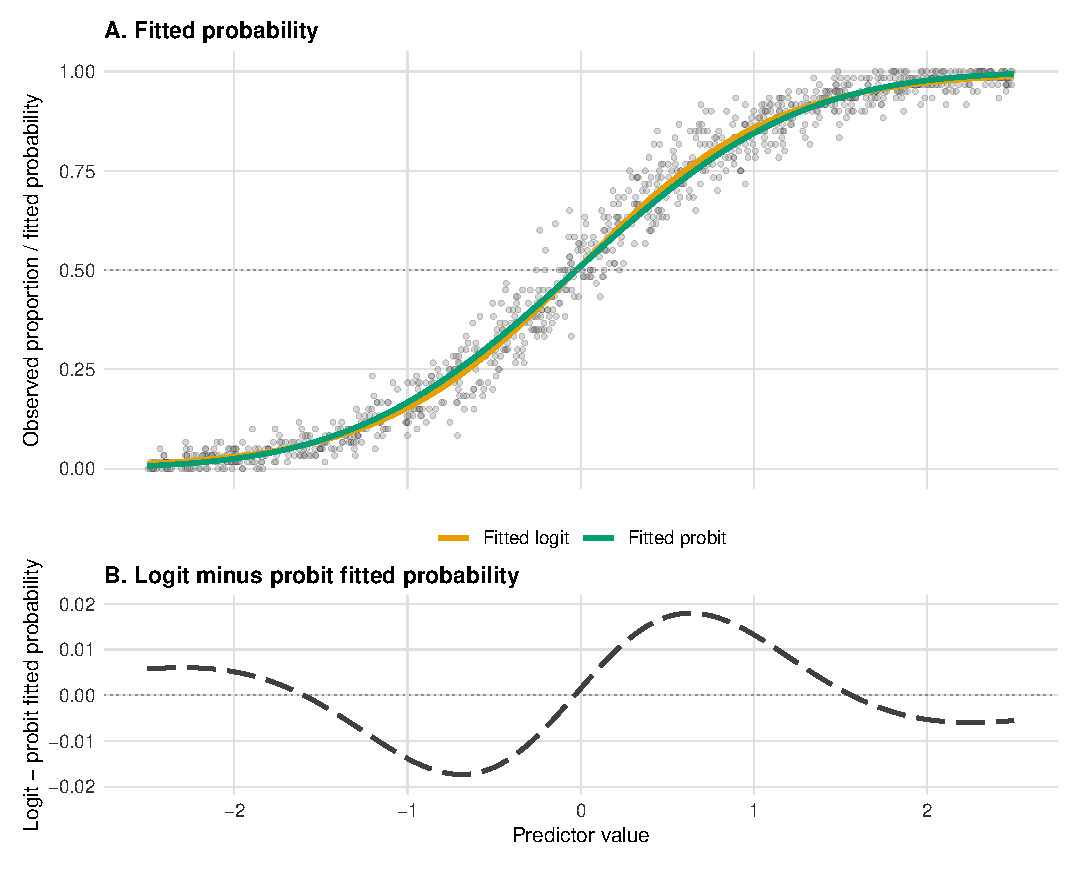
\includegraphics[width=0.8\linewidth,height=\textheight,keepaspectratio]{../figs/logit-probit-fitted-example.pdf}

}

\end{figure}%

\begin{longtable}[]{@{}llll@{}}
\caption{Coefficients and AIC for the logit and probit models fitted to
the grouped-binomial illustration dataset. Intercept and slope are on
each model's own link scale, so they are not directly comparable across
rows.}\label{tbl-logit-probit-fitted}\tabularnewline
\toprule\noalign{}
Model & Intercept & Slope & AIC \\
\midrule\noalign{}
\endfirsthead
\toprule\noalign{}
Model & Intercept & Slope & AIC \\
\midrule\noalign{}
\endhead
\bottomrule\noalign{}
\endlastfoot
logit & 0.045 & 1.753 & 4315.6 \\
probit & 0.024 & 0.990 & 4380.4 \\
\end{longtable}

\subsection{Diagnostic detection rates and AIC
strength}\label{diagnostic-detection-rates-and-aic-strength}

The main paper reports the DHARMa detection rate as a min-to-max range
across checks. Table~\ref{tbl-diagnostic-breakdown} gives the individual
checks, the within-replication alignment between pseudo-interactions and
applicable DHARMa checks, and the strength of the same-formula AIC
comparison.

\begin{longtable}[]{@{}
  >{\raggedright\arraybackslash}p{(\linewidth - 10\tabcolsep) * \real{0.4184}}
  >{\raggedright\arraybackslash}p{(\linewidth - 10\tabcolsep) * \real{0.1277}}
  >{\raggedright\arraybackslash}p{(\linewidth - 10\tabcolsep) * \real{0.1135}}
  >{\raggedright\arraybackslash}p{(\linewidth - 10\tabcolsep) * \real{0.1135}}
  >{\raggedright\arraybackslash}p{(\linewidth - 10\tabcolsep) * \real{0.1135}}
  >{\raggedright\arraybackslash}p{(\linewidth - 10\tabcolsep) * \real{0.1135}}@{}}
\caption{Diagnostic detection rates and AIC strength across five
scenarios. D1 count errors (Poisson log to identity); D2 chance-floor
accuracy (chance-corrected to standard logit); D3 binary 2x2 GLMM
(probit to logit); D4 binary continuous-predictor GLMM (probit to
logit); D5 Gamma mean response time (log to
inverse).}\label{tbl-diagnostic-breakdown}\tabularnewline
\toprule\noalign{}
\begin{minipage}[b]{\linewidth}\raggedright
Check
\end{minipage} & \begin{minipage}[b]{\linewidth}\raggedright
D1
\end{minipage} & \begin{minipage}[b]{\linewidth}\raggedright
D2
\end{minipage} & \begin{minipage}[b]{\linewidth}\raggedright
D3
\end{minipage} & \begin{minipage}[b]{\linewidth}\raggedright
D4
\end{minipage} & \begin{minipage}[b]{\linewidth}\raggedright
D5
\end{minipage} \\
\midrule\noalign{}
\endfirsthead
\toprule\noalign{}
\begin{minipage}[b]{\linewidth}\raggedright
Check
\end{minipage} & \begin{minipage}[b]{\linewidth}\raggedright
D1
\end{minipage} & \begin{minipage}[b]{\linewidth}\raggedright
D2
\end{minipage} & \begin{minipage}[b]{\linewidth}\raggedright
D3
\end{minipage} & \begin{minipage}[b]{\linewidth}\raggedright
D4
\end{minipage} & \begin{minipage}[b]{\linewidth}\raggedright
D5
\end{minipage} \\
\midrule\noalign{}
\endhead
\bottomrule\noalign{}
\endlastfoot
Pseudo-interaction (wrong link) & 2693/2790 (96.5\%) & 588 (19.6\%) &
302 (10.1\%) & 201 (6.7\%) & 918 (30.6\%) \\
DHARMa: uniformity & 0.9\% & 3.6\% & 3.1\% & 3.4\% & 0.0\% \\
DHARMa: dispersion & 21.7\% & 0.0\% & 0.0\% & 0.0\% & 0.1\% \\
DHARMa: quantiles vs fitted & 63.7\% & 1.6\% & 3.2\% & 2.0\% & 2.7\% \\
DHARMa: quantiles vs predictor & 90.9\% & 1.5\% & -- & 2.3\% & 6.4\% \\
DHARMa: across design cells & -- & -- & 0.9\% & -- & -- \\
Pseudo-interactions missed by all applicable DHARMa checks & 200/2693
(7.4\%) & 570/588 (96.9\%) & 289/302 (95.7\%) & 191/201 (95.0\%) &
853/918 (92.9\%) \\
Pregibon link check & 99.3\% & 11.9\% & N.A. & 5.4\% & 32.2\% \\
AIC favors target link & 99.3\% & 96.9\% & 95.5\% & 95.5\% & 79.7\% \\
AIC favors misspecified link & 0.7\% & 3.1\% & 4.5\% & 4.5\% & 20.3\% \\
Median ΔAIC & 22.8 (n = 2790) & 13.5 (n = 3000) & 6.0 (n = 3000) & 4.8
(n = 3000) & 2.4 (n = 3000) \\
\textbar ΔAIC\textbar{} \textless{} 2 & 23/2790 (0.8\%) & 114 (3.8\%) &
332 (11.1\%) & 431 (14.4\%) & 1142 (38.1\%) \\
\end{longtable}

Publication runs request 3,000 replications, and each table reports its
usable denominator. ``Missed'' means that none of the applicable
prespecified DHARMa checks had \(p < .05\); pseudo-interactions for
which all five DHARMa p-values were missing are excluded from this
conditional denominator.
\(\Delta\mathrm{AIC} = \mathrm{AIC}(\text{wrong link}) - \mathrm{AIC}(\text{target link})\),
so positive values favor the target link and negative values favor the
wrong link. The sample size shown with the median and the denominator
for \(|\Delta\mathrm{AIC}| < 2\) are the finite AIC comparisons. N.A.
indicates that the Pregibon-style added term is not identifiable in the
saturated \(2 \times 2\) interaction model.

\subsection{Distribution of the AIC
difference}\label{distribution-of-the-aic-difference}

The proportion of replications in which AIC favours the target link is
not informative on its own, because winning by less than one AIC unit
and winning by fifty describe different situations.
Table~\ref{tbl-diagnostic-aic-distribution} therefore gives the
distribution of \(\Delta\mathrm{AIC}\) rather than only its median. The
D2 values require regeneration after the chance-floor scenario was
converted to the subject-random-intercept design.

\begin{longtable}[]{@{}
  >{\raggedright\arraybackslash}p{(\linewidth - 16\tabcolsep) * \real{0.3146}}
  >{\raggedleft\arraybackslash}p{(\linewidth - 16\tabcolsep) * \real{0.0562}}
  >{\raggedright\arraybackslash}p{(\linewidth - 16\tabcolsep) * \real{0.0562}}
  >{\raggedright\arraybackslash}p{(\linewidth - 16\tabcolsep) * \real{0.0562}}
  >{\raggedright\arraybackslash}p{(\linewidth - 16\tabcolsep) * \real{0.0787}}
  >{\raggedright\arraybackslash}p{(\linewidth - 16\tabcolsep) * \real{0.0562}}
  >{\raggedright\arraybackslash}p{(\linewidth - 16\tabcolsep) * \real{0.0562}}
  >{\raggedright\arraybackslash}p{(\linewidth - 16\tabcolsep) * \real{0.1685}}
  >{\raggedright\arraybackslash}p{(\linewidth - 16\tabcolsep) * \real{0.1573}}@{}}
\caption{Distribution of the AIC difference across replications, by
diagnostic scenario. Delta AIC = AIC(wrong link) - AIC(target link), so
positive values favor the target link. n = replications with both AIC
values available.}\label{tbl-diagnostic-aic-distribution}\tabularnewline
\toprule\noalign{}
\begin{minipage}[b]{\linewidth}\raggedright
Scenario
\end{minipage} & \begin{minipage}[b]{\linewidth}\raggedleft
n
\end{minipage} & \begin{minipage}[b]{\linewidth}\raggedright
10th
\end{minipage} & \begin{minipage}[b]{\linewidth}\raggedright
25th
\end{minipage} & \begin{minipage}[b]{\linewidth}\raggedright
Median
\end{minipage} & \begin{minipage}[b]{\linewidth}\raggedright
75th
\end{minipage} & \begin{minipage}[b]{\linewidth}\raggedright
90th
\end{minipage} & \begin{minipage}[b]{\linewidth}\raggedright
Within 2 units
\end{minipage} & \begin{minipage}[b]{\linewidth}\raggedright
Favors target
\end{minipage} \\
\midrule\noalign{}
\endfirsthead
\toprule\noalign{}
\begin{minipage}[b]{\linewidth}\raggedright
Scenario
\end{minipage} & \begin{minipage}[b]{\linewidth}\raggedleft
n
\end{minipage} & \begin{minipage}[b]{\linewidth}\raggedright
10th
\end{minipage} & \begin{minipage}[b]{\linewidth}\raggedright
25th
\end{minipage} & \begin{minipage}[b]{\linewidth}\raggedright
Median
\end{minipage} & \begin{minipage}[b]{\linewidth}\raggedright
75th
\end{minipage} & \begin{minipage}[b]{\linewidth}\raggedright
90th
\end{minipage} & \begin{minipage}[b]{\linewidth}\raggedright
Within 2 units
\end{minipage} & \begin{minipage}[b]{\linewidth}\raggedright
Favors target
\end{minipage} \\
\midrule\noalign{}
\endhead
\bottomrule\noalign{}
\endlastfoot
Count errors & 2790 & 10.7 & 16.6 & 22.8 & 30.3 & 36.4 & 0.8\% &
99.3\% \\
Chance-floor accuracy & 3000 & 4.3 & 8.5 & 13.5 & 19.0 & 24.2 & 3.8\% &
96.9\% \\
Binary repeated trials & 3000 & 1.5 & 3.8 & 6.0 & 8.4 & 10.5 & 11.1\% &
95.5\% \\
Binary continuous predictor & 3000 & 1.2 & 3.0 & 4.8 & 6.8 & 8.5 &
14.4\% & 95.5\% \\
Gamma mean response time & 3000 & -1.3 & 0.4 & 2.4 & 4.5 & 6.3 & 38.1\%
& 79.7\% \\
\end{longtable}

\subsection{Calibration under correctly specified
links}\label{calibration-under-correctly-specified-links}

The same DHARMa and Pregibon-style checks were applied to the
corresponding correct-link interaction model in each replication. These
baseline flagging rates provide a reference for interpreting detection
under the wrong link. They reuse the same simulated datasets and
scenarios rather than defining a new simulation.

The correct-link column provides the baseline needed to interpret
detection under the wrong link. The four DHARMa checks are well
calibrated throughout. For the Pregibon-style check, the
random-intercept GLMMs use the population-level rather than
subject-specific fitted linear predictor. The \(2 \times 2\) version is
not applicable because its saturated fixed-effects design already spans
the proposed squared term; the continuous-predictor version is
estimable, and its wrong-link flagging rate should be read against its
correct-link calibration rate.

\begin{longtable}[]{@{}
  >{\raggedright\arraybackslash}p{(\linewidth - 6\tabcolsep) * \real{0.2171}}
  >{\raggedright\arraybackslash}p{(\linewidth - 6\tabcolsep) * \real{0.3798}}
  >{\raggedright\arraybackslash}p{(\linewidth - 6\tabcolsep) * \real{0.1705}}
  >{\raggedright\arraybackslash}p{(\linewidth - 6\tabcolsep) * \real{0.2326}}@{}}
\caption{Diagnostic calibration under correctly specified and
misspecified links. Each cell gives the flagging rate with its Wilson
95\% confidence interval and the number of successful diagnostic fits.
Each cell had 3,000 attempted
replications.}\label{tbl-diagnostic-calibration}\tabularnewline
\toprule\noalign{}
\begin{minipage}[b]{\linewidth}\raggedright
Scenario
\end{minipage} & \begin{minipage}[b]{\linewidth}\raggedright
Diagnostic
\end{minipage} & \begin{minipage}[b]{\linewidth}\raggedright
Correct-link flagging
\end{minipage} & \begin{minipage}[b]{\linewidth}\raggedright
Wrong-link flagging
\end{minipage} \\
\midrule\noalign{}
\endfirsthead
\toprule\noalign{}
\begin{minipage}[b]{\linewidth}\raggedright
Scenario
\end{minipage} & \begin{minipage}[b]{\linewidth}\raggedright
Diagnostic
\end{minipage} & \begin{minipage}[b]{\linewidth}\raggedright
Correct-link flagging
\end{minipage} & \begin{minipage}[b]{\linewidth}\raggedright
Wrong-link flagging
\end{minipage} \\
\midrule\noalign{}
\endhead
\bottomrule\noalign{}
\endlastfoot
Count errors & DHARMa uniformity & 0.1\% {[}0.0, 0.2{]} & 0.9\% {[}0.6,
1.3{]} (n = 2790) \\
Count errors & DHARMa dispersion & 5.3\% {[}4.5, 6.1{]} & 21.7\%
{[}20.2, 23.3{]} (n = 2790) \\
Count errors & DHARMa residual quantiles over fitted values & 3.4\%
{[}2.8, 4.1{]} & 63.7\% {[}61.9, 65.5{]} (n = 2790) \\
Count errors & DHARMa residual quantiles over focal predictor & 3.9\%
{[}3.3, 4.7{]} & 90.9\% {[}89.8, 91.9{]} (n = 2790) \\
Count errors & Pregibon-style added-term link check & 4.7\% {[}4.0,
5.5{]} & 99.3\% {[}98.9, 99.5{]} (n = 2790) \\
Chance-floor accuracy & DHARMa uniformity & 37.5\% {[}35.8, 39.3{]} &
3.6\% {[}3.0, 4.4{]} \\
Chance-floor accuracy & DHARMa dispersion & 35.8\% {[}34.1, 37.5{]} &
0.0\% {[}0.0, 0.1{]} \\
Chance-floor accuracy & DHARMa residual quantiles over fitted values &
8.9\% {[}8.0, 10.0{]} & 1.6\% {[}1.2, 2.2{]} \\
Chance-floor accuracy & DHARMa residual quantiles over focal predictor &
8.7\% {[}7.8, 9.8{]} & 1.5\% {[}1.1, 2.0{]} \\
Chance-floor accuracy & Pregibon-style added-term link check & 43.1\%
{[}41.4, 44.9{]} & 11.9\% {[}10.8, 13.1{]} \\
Binary repeated trials & DHARMa uniformity & 3.8\% {[}3.2, 4.5{]} &
3.1\% {[}2.5, 3.8{]} \\
Binary repeated trials & DHARMa dispersion & 0.0\% {[}0.0, 0.1{]} &
0.0\% {[}0.0, 0.1{]} \\
Binary repeated trials & DHARMa residual quantiles over fitted values &
3.1\% {[}2.5, 3.8{]} & 3.2\% {[}2.6, 3.9{]} \\
Binary repeated trials & DHARMa residual distribution across design
cells & 0.8\% {[}0.5, 1.1{]} & 0.9\% {[}0.6, 1.3{]} \\
Binary repeated trials & Pregibon-style added-term link check & N.A. &
N.A. \\
Binary continuous predictor & DHARMa uniformity & 3.9\% {[}3.3, 4.7{]} &
3.4\% {[}2.8, 4.1{]} \\
Binary continuous predictor & DHARMa dispersion & 0.0\% {[}0.0, 0.1{]} &
0.0\% {[}0.0, 0.1{]} \\
Binary continuous predictor & DHARMa residual quantiles over fitted
values & 3.0\% {[}2.5, 3.7{]} & 2.0\% {[}1.6, 2.6{]} \\
Binary continuous predictor & DHARMa residual quantiles over focal
predictor & 2.5\% {[}2.0, 3.2{]} & 2.3\% {[}1.8, 2.9{]} \\
Binary continuous predictor & Pregibon-style added-term link check &
5.3\% {[}4.5, 6.1{]} & 5.4\% {[}4.7, 6.3{]} \\
Gamma mean response time & DHARMa uniformity & 0.0\% {[}0.0, 0.1{]} &
0.0\% {[}0.0, 0.2{]} \\
Gamma mean response time & DHARMa dispersion & 0.4\% {[}0.2, 0.7{]} &
0.1\% {[}0.1, 0.3{]} \\
Gamma mean response time & DHARMa residual quantiles over fitted values
& 1.5\% {[}1.1, 2.0{]} & 2.7\% {[}2.2, 3.4{]} \\
Gamma mean response time & DHARMa residual quantiles over focal
predictor & 2.3\% {[}1.8, 2.9{]} & 6.4\% {[}5.6, 7.4{]} \\
Gamma mean response time & Pregibon-style added-term link check & 4.0\%
{[}3.4, 4.8{]} & 32.2\% {[}30.6, 33.9{]} \\
\end{longtable}

\subsection{Deterministic pseudo-interaction under the wrong
link}\label{deterministic-pseudo-interaction-under-the-wrong-link}

Figure~\ref{fig-within-family-inspection} shows the deterministic
pseudo-interaction induced on the wrong link scale in Simulation 2,
before any sampling noise. It makes explicit why matched-link cells
imply an exactly additive structure while wrong-link cells do not.

\begin{figure}[H]

\caption{\label{fig-within-family-inspection}Deterministic
pseudo-interaction induced on the wrong link scale in Simulation 2.}

\centering{

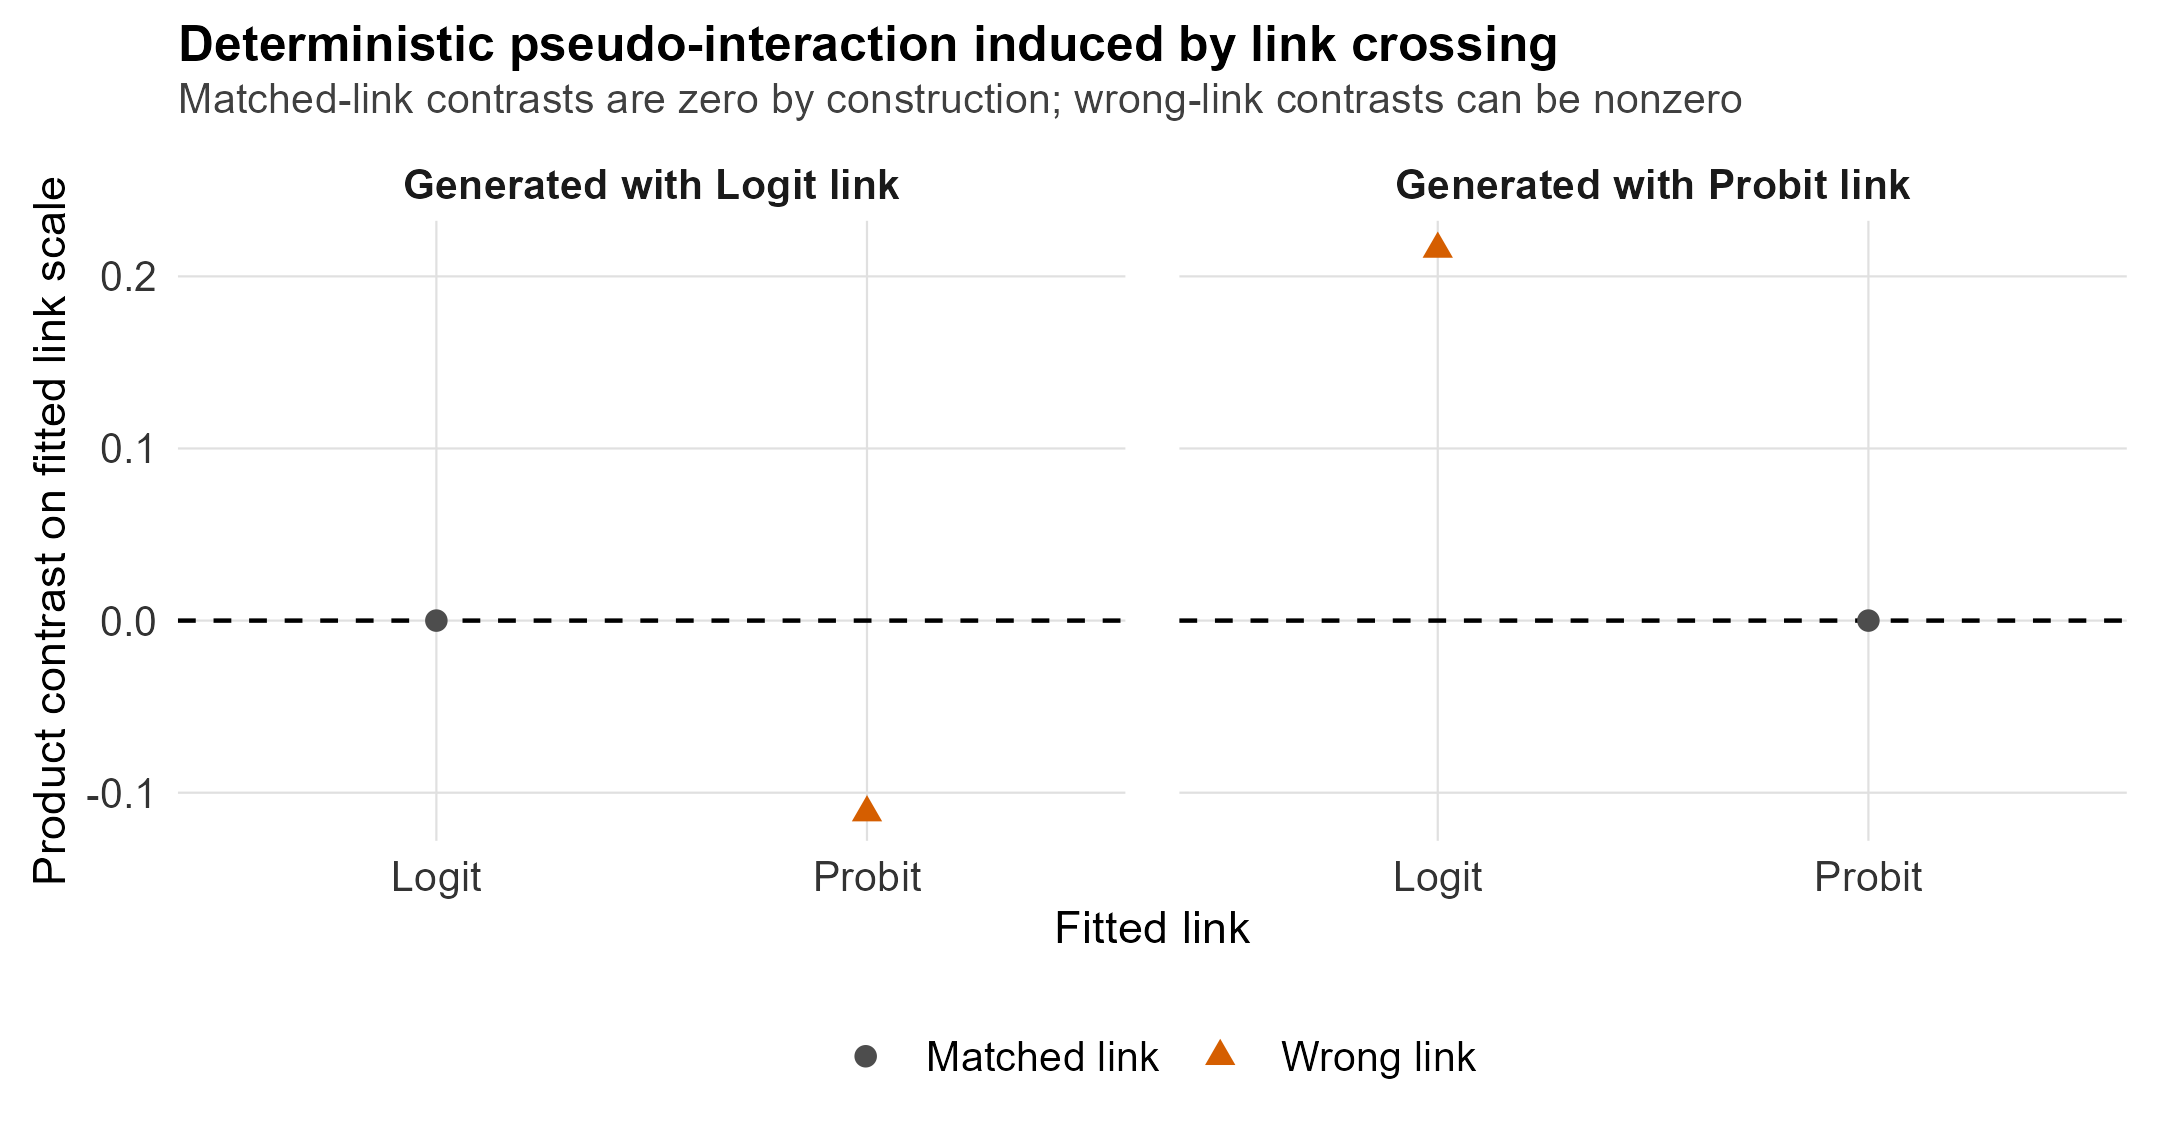
\includegraphics[width=0.95\linewidth,height=\textheight,keepaspectratio]{../outputs/inspection/within-family-link-pseudo-interaction.png}

}

\end{figure}%

\section{S6. Data, code, and computational
environment}\label{s6.-data-code-and-computational-environment}

All analyses were conducted in R, and the manuscript and this supplement
were written in Quarto. Each simulation sets a fixed random seed, and
the number of Monte Carlo replications and the significance level are
recorded together with the saved results. Exact package versions are
pinned with \texttt{renv}, which is the source of truth for the
computational environment; the key modelling dependencies are
\texttt{glmmTMB} for the mixed-model simulations and \texttt{DHARMa} for
the diagnostic checks. The complete data, analysis code, preregistration
materials, and generated outputs are archived in the public repository
associated with the article, so that every table and figure can be
regenerated from the raw inputs.

The manuscript simulations use a small number of transparent scenarios.
A broader precomputed sensitivity atlas generated in
\texttt{simulation-atlas/} varies key parameters around those anchors,
and the Shiny app explores its compact summaries without running
simulations interactively. Replication-level atlas results are intended
for the public repository or OSF archive and are not required to render
this supplement.

\section{References}\label{references}

\protect\phantomsection\label{refs}
\begin{CSLReferences}{1}{0}
\bibitem[\citeproctext]{ref-dunnsmyth1996}
Dunn, P. K., \& Smyth, G. K. (1996). Randomized quantile residuals.
\emph{Journal of Computational and Graphical Statistics}, \emph{5}(3),
236--244. \url{https://doi.org/10.1080/10618600.1996.10474708}

\bibitem[\citeproctext]{ref-hartig2024}
Hartig, F. (2024). \emph{{DHARMa}: Residual diagnostics for hierarchical
(multi-level / mixed) regression models}.
\url{https://doi.org/10.32614/CRAN.package.DHARMa}

\bibitem[\citeproctext]{ref-knoblauch2012}
Knoblauch, K., \& Maloney, L. T. (2012). \emph{Modeling psychophysical
data in r}. Springer. \url{https://doi.org/10.1007/978-1-4614-4475-6}

\bibitem[\citeproctext]{ref-pregibon1980}
Pregibon, D. (1980). Goodness of link tests for generalized linear
models. \emph{Journal of the Royal Statistical Society Series C: Applied
Statistics}, \emph{29}(1), 15--24. \url{https://doi.org/10.2307/2346405}

\bibitem[\citeproctext]{ref-wichmann2001}
Wichmann, F. A., \& Hill, N. J. (2001). The psychometric function: I.
Fitting, sampling, and goodness of fit. \emph{Perception \&
Psychophysics}, \emph{63}(8), 1293--1313.
\url{https://doi.org/10.3758/BF03194544}

\end{CSLReferences}






\end{document}
